\documentclass[12pt,a4paper]{report}
\usepackage[T1]{fontenc}
\usepackage[utf8]{inputenc}
\usepackage{newtxtext,newtxmath}
\usepackage[top=1in,bottom=0.8in,left=1.5in,right=1in]{geometry}
\usepackage{setspace}
\usepackage{microtype}
\usepackage{graphicx,tabularx,booktabs,multirow,amsmath,siunitx,pdflscape,subcaption,float,listings}
\usepackage[font=small,labelfont=bf]{caption}
\usepackage{titlesec,fancyhdr,etoolbox,array}
\usepackage[hidelinks]{hyperref}
\usepackage{tocloft}

\newcommand{\aicad}{\textsf{aicad}}
\newcommand{\NChecks}{44}
\newcommand{\NTests}{301}
\newcommand{\WorstMin}{71}
\newcommand{\WorstMax}{79}
\newcommand{\KnuckleRod}{35}
\newcommand{\KnucklePin}{45}
\newcommand{\BhandariMatch}{9}
\newcommand{\BhandariOf}{9}
\newcommand{\SizingLoad}{62{,}500}


% -- text: 1.5 spacing, justified
\onehalfspacing
\setlength{\parindent}{10mm}
\setlength{\parskip}{0pt}
\setlength{\emergencystretch}{3em}
\captionsetup[table]{position=above,skip=4pt}
\captionsetup[figure]{position=below,skip=4pt}
\renewcommand{\arraystretch}{1.1}
\setlength{\tabcolsep}{4pt}

% -- chapter title page: number and title alone, right aligned, 14 pt bold upper case
\titleformat{\chapter}[display]{\raggedleft\fontsize{14}{20}\selectfont\bfseries}
  {\MakeUppercase{\chaptertitlename}\ \thechapter}{6mm}
  {\expandafter\gdef\csname tp@\thepage\endcsname{}\fontsize{14}{20}\selectfont\bfseries\MakeUppercase}[\clearpage]

\titlespacing{\chapter}{0pt}{30mm}{0pt}
\titleformat{name=\chapter,numberless}[block]{\centering\fontsize{16}{20}\selectfont\bfseries}{}{0pt}{\underline}
\titlespacing{name=\chapter,numberless}{0pt}{0pt}{8pt}
\titleformat{\section}{\normalfont\fontsize{12}{14}\selectfont\bfseries}{\thesection}{1em}{}
\titleformat{\subsection}{\normalfont\fontsize{12}{14}\selectfont\bfseries}{\thesubsection}{1em}{}
\titlespacing*{\section}{0pt}{10pt}{4pt}
\titlespacing*{\subsection}{0pt}{8pt}{3pt}
\renewcommand{\thetable}{\thechapter.\arabic{table}}
\renewcommand{\thefigure}{\thechapter.\arabic{figure}}
\renewcommand{\theequation}{\thechapter.\arabic{equation}}
\setcounter{secnumdepth}{2}
\setcounter{tocdepth}{1}

% -- header and footer: one definition used for fancy and plain, so a chapter's first page
% (which LaTeX forces to plain) differs only by the suppressed header
\newcommand{\hdr}{}
\newcommand{\hdrfoot}{\fancyhf{}\renewcommand{\headrulewidth}{0pt}\renewcommand{\footrulewidth}{0pt}
  \fancyhead[R]{\fontsize{10}{12}\selectfont\ifcsname tp@\thepage\endcsname\else\hdr\fi}
  \fancyfoot[L]{\fontsize{10}{12}\selectfont Department of Mechanical Engineering}
  \fancyfoot[C]{\fontsize{10}{12}\selectfont\thepage}
  \fancyfoot[R]{\fontsize{10}{12}\selectfont S.G.S.I.T.S., Indore}}
\pagestyle{fancy}\hdrfoot
\fancypagestyle{plain}{\hdrfoot}
\fancypagestyle{empty}{\fancyhf{}\renewcommand{\headrulewidth}{0pt}\renewcommand{\footrulewidth}{0pt}}
\renewcommand{\chaptermark}[1]{\markboth{#1}{}}
\setlength{\headheight}{14pt}

% -- code listings
\lstset{basicstyle=\ttfamily\fontsize{8}{9}\selectfont,numbers=left,numberstyle=\tiny,numbersep=5pt,
  breaklines=true,breakatwhitespace=false,columns=fullflexible,keepspaces=true,frame=single,
  xleftmargin=1.2em,framexleftmargin=1.2em,aboveskip=4pt,belowskip=2pt,
  postbreak=\mbox{\textcolor{gray}{$\hookrightarrow$}\space}}
\usepackage{xcolor}

\newcommand{\fmhead}[1]{\begin{center}{\fontsize{16}{20}\selectfont\bfseries\underline{#1}}\end{center}\vspace{2mm}}
\newcommand{\toctoc}[1]{\clearpage\phantomsection\addcontentsline{toc}{chapter}{#1}}

% institute heading used above the recommendation and the certificate
\newcommand{\insthead}{%
  \begin{center}
  {\fontsize{14}{17}\selectfont\bfseries SHRI G.S. INSTITUTE OF TECHNOLOGY AND SCIENCE, INDORE (M.P.)}\\[1mm]
  A Govt.\ Aided Autonomous Institute, Affiliated to RGPV, Bhopal\\[1mm]
  {\fontsize{14}{17}\selectfont\bfseries DEPARTMENT OF MECHANICAL ENGINEERING}\\[2mm]
  
\includegraphics[width=22mm]{fig/sgsits-logo.png}\\[1mm]
  {\fontsize{14}{17}\selectfont\bfseries 2026 -- 2027}
  \end{center}}

\newcommand{\projtitle}{Strategic Application of Artificial Intelligence in CAD}
\newcommand{\teamnames}{Ankur Dodke, Ansh Yadav, Atishay Jain, Bhavya Shrivastava, Dharmendra Gupta}

\usepackage{enumitem}
\setlist{nosep,leftmargin=*}
\begin{document}
\pagenumbering{roman}
\setcounter{page}{0}

% ----------------------------------------------------------------- cover (counted, not printed)
\thispagestyle{empty}
\begin{center}\singlespacing
{\fontsize{18}{23}\selectfont\bfseries STRATEGIC APPLICATION OF ARTIFICIAL INTELLIGENCE IN CAD\par}
\vspace{8mm}

\includegraphics[width=28mm]{fig/sgsits-logo.png}\par
\vspace{8mm}
{\fontsize{14}{17}\selectfont\bfseries\itshape A Project Report Submitted to\\
Rajiv Gandhi Proudyogiki Vishwavidyalaya, Bhopal\\
towards the partial fulfillment of the degree of Bachelor of Technology\\
in Mechanical Engineering\par}
\vspace{8mm}
{\fontsize{16}{20}\selectfont\bfseries 2026 -- 2027\par}
\vspace{10mm}
\noindent\begin{minipage}[t]{0.42\textwidth}\raggedright
{\fontsize{14}{17}\selectfont\bfseries Supervised by:}\\[2mm]
Dr.\ B.\ R.\ Rawal\\Professor and Head\\Department of Mechanical Engineering
\end{minipage}\hfill
\begin{minipage}[t]{0.54\textwidth}\raggedleft
{\fontsize{14}{17}\selectfont\bfseries Submitted by:}\\[2mm]
\begin{tabular}{@{}r@{\hspace{4mm}}l@{}}
0801ME231013 & Ankur Dodke\\
0801ME231014 & Ansh Yadav\\
0801ME231024 & Atishay Jain\\
0801ME231030 & Bhavya Shrivastava\\
0801ME243D02 & Dharmendra Gupta
\end{tabular}
\end{minipage}
\vfill
{\fontsize{14}{17}\selectfont\bfseries SHRI G.S. INSTITUTE OF TECHNOLOGY AND SCIENCE,\\ INDORE (M.P.)\par}
{\normalsize A Govt.\ Aided Autonomous Institute, Affiliated to RGPV, Bhopal\par}
\end{center}

% ----------------------------------------------------------------- recommendation, certificate
\clearpage\phantomsection\addcontentsline{toc}{chapter}{Recommendation}
\insthead\fmhead{RECOMMENDATION}
{\fontsize{12}{17}\selectfont\bfseries\noindent We are pleased to recommend that the project work entitled
\textit{\projtitle} submitted by \teamnames{} may be accepted in partial fulfillment of the degree of
Bachelor of Technology in Mechanical Engineering of Rajiv Gandhi Proudyogiki Vishwavidyalaya,
Bhopal (M.P.) during the session 2026 -- 2027.\par}
\vspace{8mm}\singlespacing\noindent\bfseries
\begin{tabular}[t]{@{}l@{}}Dr.\ B.\ R.\ Rawal\\Professor and Head\\Department of Mechanical Engineering\end{tabular}\hfill
\begin{tabular}[t]{@{}l@{}}Head of Department\\Professor and Head\\Department of Mechanical Engineering\end{tabular}
\onehalfspacing\normalfont

\vspace{6mm}\phantomsection\addcontentsline{toc}{chapter}{Certificate}
\fmhead{CERTIFICATE}
{\fontsize{12}{17}\selectfont\bfseries\noindent This is to certify that the Project entitled \textit{\projtitle}
submitted by \teamnames{} is accepted in partial fulfillment of the degree of Bachelor of Technology
in Mechanical Engineering of Rajiv Gandhi Proudyogiki Vishwavidyalaya, Bhopal during the session
2026 -- 2027.\par}
\vspace{14mm}\noindent\bfseries
\begin{tabular}[t]{@{}c@{}}\rule{55mm}{0.6pt}\\Internal Examiner\\Date:\ \rule{25mm}{0.4pt}\end{tabular}\hfill
\begin{tabular}[t]{@{}c@{}}\rule{55mm}{0.6pt}\\External Examiner\\Date:\ \rule{25mm}{0.4pt}\end{tabular}
\normalfont

% ----------------------------------------------------------------- declaration
\toctoc{Declaration}
\fmhead{DECLARATION}
\noindent We, the undersigned students of the final year Bachelor of Technology course in
Mechanical Engineering, Department of Mechanical Engineering, Shri G.S. Institute of Technology
and Science, Indore (M.P.), declare that the project entitled \textit{\projtitle} is our own work
conducted under the supervision of Dr.\ B.\ R.\ Rawal, Professor and Head, Department of
Mechanical Engineering, Shri G.\ S.\ Institute of Technology and Science, Indore.

\noindent\hspace{10mm}We affirm that this work is entirely original and has not been copied from any
source. All sources consulted during the work have been duly acknowledged and cited in the
references. Every design formula and empirical proportion used in the software developed for this
project is attributed in the text to the published source from which it is taken, and every
instance in which the software departs from a cited source is stated explicitly in Chapter 7
together with the reason for the departure.

\hspace{10mm}We further declare that, to the best of our knowledge, this project work does not
contain any part of any work which has been submitted for the award of any degree either in this
University or in any other University or from any website without proper citation.

\vspace{14mm}\singlespacing\footnotesize\noindent
\begin{tabularx}{\textwidth}{*{5}{>{\centering\arraybackslash}X}}
\rule{0.9\linewidth}{0.5pt} & \rule{0.9\linewidth}{0.5pt} & \rule{0.9\linewidth}{0.5pt} &
\rule{0.9\linewidth}{0.5pt} & \rule{0.9\linewidth}{0.5pt}\\
Signature of the candidate & Signature of the candidate & Signature of the candidate &
Signature of the candidate & Signature of the candidate\\
Date & Date & Date & Date & Date\\[3mm]
\textbf{Ankur Dodke} 0801ME231013 & \textbf{Ansh Yadav} 0801ME231014 &
\textbf{Atishay Jain} 0801ME231024 & \textbf{Bhavya Shrivastava} 0801ME231030 &
\textbf{Dharmendra Gupta} 0801ME243D02
\end{tabularx}
\normalsize\onehalfspacing

% ----------------------------------------------------------------- acknowledgement
\toctoc{Acknowledgement}
\fmhead{ACKNOWLEDGEMENT}
\noindent We express our sincere gratitude to Dr.\ B.\ R.\ Rawal, Professor and Head, Department of
Mechanical Engineering, for the guidance and encouragement extended throughout this work. The
direction to keep every computed dimension traceable to a published formula, rather than to a
convenient result, shaped this project more than any other single input, and it is the reason the
verification exercise reported in Chapter 7 was carried out at all.

\hspace{10mm}We thank the faculty of the Department of Mechanical Engineering for their observations
during the review presentations, which repeatedly sharpened the scope of the work, and the
Institute for providing the facilities and the academic environment in which the work was carried
out.

\hspace{10mm}We acknowledge the National Programme on Technology Enhanced Learning and the Indian
Institute of Technology Kharagpur, whose openly published course material on the design of machine
elements is the primary reference for this work, and the Internet Archive, through which the out of
copyright texts by Unwin and by Leutwiler were obtained.

\hspace{10mm}Finally, we thank our families and our classmates for their support during the course of
this project.

\vspace{10mm}\begin{flushright}\singlespacing
Ankur Dodke (0801ME231013)\\Ansh Yadav (0801ME231014)\\Atishay Jain (0801ME231024)\\
Bhavya Shrivastava (0801ME231030)\\Dharmendra Gupta (0801ME243D02)\\[3mm]
Date:\ \rule{30mm}{0.4pt}\end{flushright}\onehalfspacing

% ----------------------------------------------------------------- abstract
\toctoc{Abstract}
\fmhead{ABSTRACT}
\noindent Designing a standard machine joint is a repetitive calculation. For a knuckle joint the
designer computes the rod diameter from direct tension, sizes the pin separately for double shear
and for bending, adopts the larger of the two requirements, derives the remaining proportions from
the rod diameter, and then verifies nine distinct failure modes against allowable stresses. A change
in the applied load invalidates every one of those results and requires the entire sequence again.
Computer aided design software removes the labour of drawing but not the labour of calculation: a
modeller regenerates whatever dimensions it is given and will not object if a pin is too slender to
carry the bending moment placed upon it.

\hspace{10mm}This project presents a software system that performs the complete sequence
automatically from a requirement written in ordinary English. The user enters a sentence such as
\textit{knuckle joint for 50 kN}. A language model extracts the parameters from that sentence. All
subsequent work is deterministic: the joint is sized from standard design formulas, each computed
diameter is rounded up to the next preferred size and each derived thickness to the next whole
millimetre, every applicable failure mode is verified against the allowable stress, any dimension
that fails is increased until it passes, every component is generated as an exact solid model, and a
first angle A3 drawing sheet is produced with dimension lines and a title block.

\hspace{10mm}Six joints are implemented: the knuckle joint, the socket and spigot cotter joint, the
sleeve and cotter joint, the gib and cotter joint, the hex bolted joint and the protected type rigid
flange coupling. Together they apply \NChecks{} distinct failure checks. Every proportion and every
check was compared against published design literature, and the comparison identified three errors
in the sources themselves, including a worked example whose own answer exceeds its own allowable
stress by 23 percent. The implementation is covered by \NTests{} automated tests and is deployed as
a web application requiring no installation.

\hspace{10mm}The central design decision is that the language model reads the requirement only. It
selects no dimension and performs no check. Interpreting a phrase is a problem of language;
selecting a pin diameter is a problem of engineering with a single correct answer, and it remains
with deterministic code whose every step can be traced to a printed page.

% ----------------------------------------------------------------- contents and lists
\clearpage\singlespacing
\phantomsection\addcontentsline{toc}{chapter}{Table of Contents}
\renewcommand{\contentsname}{TABLE OF CONTENTS}
\renewcommand{\cftchapfont}{\small\bfseries}
\renewcommand{\cftchappagefont}{\bfseries}
\setlength{\cftbeforechapskip}{2pt}
\setlength{\cftbeforesecskip}{0pt}
\renewcommand{\cftchapdotsep}{\cftdotsep}
\renewcommand{\cftsecfont}{\footnotesize}\renewcommand{\cftsecpagefont}{\footnotesize}
\setlength{\cftsecindent}{9mm}\setlength{\cftsecnumwidth}{9mm}
\setlength{\cftchapnumwidth}{9mm}
\renewcommand{\cftchappresnum}{}
\renewcommand{\cftfigfont}{\footnotesize}\renewcommand{\cfttabfont}{\footnotesize}
\renewcommand{\cftfigpresnum}{Figure~}\renewcommand{\cfttabpresnum}{Table~}
\setlength{\cftfignumwidth}{18mm}\setlength{\cfttabnumwidth}{15mm}
\setlength{\cftbeforefigskip}{2pt}\setlength{\cftbeforetabskip}{2pt}
\tableofcontents
\vspace{4mm}
\phantomsection\addcontentsline{toc}{chapter}{List of Figures}
\renewcommand{\listfigurename}{LIST OF FIGURES}
\listoffigures
\vspace{4mm}
\phantomsection\addcontentsline{toc}{chapter}{List of Tables}
\renewcommand{\listtablename}{LIST OF TABLES}
\listoftables
\vspace{4mm}
\phantomsection\addcontentsline{toc}{chapter}{List of Symbols and Abbreviations}
\fmhead{LIST OF SYMBOLS}
\footnotesize
\begin{tabularx}{\textwidth}{@{}l X l@{}}
\toprule Symbol & Meaning & Unit\\\midrule
$P$ & Applied axial load & N\\
$T$ & Transmitted torque & N\,mm\\
$D$ & Rod diameter & mm\\
$d$ & Pin or spigot diameter & mm\\
$d_2$ & Outer diameter of the eye or socket & mm\\
$t$ & Thickness of the eye, or of the cotter & mm\\
$t_1$ & Thickness of each fork plate & mm\\
$b$ & Breadth of the cotter and gib & mm\\
$\sigma_t$ & Allowable tensile stress & MPa\\
$\sigma_b$ & Allowable bending stress & MPa\\
$\sigma_c$ & Allowable crushing stress & MPa\\
$\tau$ & Allowable shear stress & MPa\\
\bottomrule\end{tabularx}
\fmhead{LIST OF ABBREVIATIONS}
\begin{tabularx}{\textwidth}{@{}l X@{}}
\toprule Abbreviation & Expansion\\\midrule
CAD & Computer Aided Design\\
STEP & Standard for the Exchange of Product data\\
DXF & Drawing Exchange Format\\
FEA & Finite Element Analysis\\
NPTEL & National Programme on Technology Enhanced Learning\\
OCCT & Open CASCADE Technology\\
BIS & Bureau of Indian Standards\\
MPa & Megapascal, newton per square millimetre\\
\bottomrule\end{tabularx}
\normalsize\onehalfspacing

% ----------------------------------------------------------------- chapters
\clearpage
\pagenumbering{arabic}\renewcommand{\hdr}{\leftmark}
\newcommand{\inchapter}[1]{\IfFileExists{#1.tex}{\include{#1}}{\chapter{Placeholder #1}}}
\IfFileExists{ch1.tex}{\chapter{Introduction}

\section{Background}
The standard joints of machine design, such as the knuckle joint, the cotter joint and the shaft coupling, are not designed by judgement: each is sized by a fixed sequence of formulas and verified against a fixed list of failure modes, as in Bhandari. The sequence is repetitive, since a change in load invalidates every dimension. Computer aided design software removes the labour of drawing but not of calculation; a parametric modeller does not object if a pin is too slender for the bending moment upon it.

\section{Motivation}
The motivation is the gap between stating a requirement and obtaining a verified design. At present a designer must translate a requirement such as \emph{a knuckle joint to carry 50 kN} into formulas by hand, check several failure modes, iterate wherever a check fails, and only then begin modelling and drafting.

A system that accepts the requirement as written and returns a verified design, with solid models and a drawing sheet, would remove the repetition without removing the engineering, provided the calculation itself stays checkable.

\section{Objectives}
The objectives of the present work are as follows.
\begin{enumerate}
  \item To develop a system that accepts a design requirement in ordinary English and extracts the joint type, the applied load and the allowable stresses.
  \item To size the joint using established design formulas and verify every applicable failure mode against the allowable stress, iterating wherever a check is not satisfied.
  \item To generate exact solid models of every component and of the assembly in a neutral exchange format that opens in commercial CAD software.
  \item To generate a first angle projection drawing sheet carrying dimensions and a title block in conformity with Indian drawing practice.
  \item To verify every proportion and failure check used by the system against published design literature, recording any disagreement with a source explicitly.
  \item To make the system usable through a web browser without any installation.
\end{enumerate}

\section{Scope of the Work}
The work covers six standard joints under static loading. Fatigue, stress concentration factors, tolerances and fits, and manufacturing processes are outside its scope; the finite element facility is a single linear static cross check, not a complete analysis.

\section{Organisation of the Report}
Chapters 2 to 4 review the literature, state the problem and describe the case studies; Chapters 5 and 6 give the methodology and its implementation; Chapter 7 presents the results and their verification, and Chapter 8 concludes.
}{\chapter{Introduction}}
\IfFileExists{ch2.tex}{\chapter{Literature Review}

\section{Design of Cotter and Knuckle Joints}

The course text, Bhandari's \textit{Design of Machine Elements}, treats the cotter joint and the knuckle joint in sections 4.9 to 4.12. It gives the strength equations for every failure mode, the empirical proportions of each joint, and complete worked examples: Examples 4.2 and 4.4 for the cotter joint and Example 4.5 for the knuckle joint. The software follows Bhandari's proportions for the knuckle joint, in which the outside diameter of the eye and the pin head are taken from the pin diameter ($d_0 = 2d$, $1.5d$) and the rod is enlarged to $1.1D$ at the eye. For the cotter joint it follows his procedure, in which the spigot and the socket are sized from their own tension equations. These worked examples are the cases against which the software is tested in Chapter 7.

A second reference is the Design of Machine Elements course published by IIT Kharagpur through NPTEL. Module 4 treats pin joints, keys and threaded fasteners, and Lesson 2 gives the complete design procedure for the socket and spigot cotter joint and for the knuckle joint, including the empirical proportions as multiples of the rod diameter and the full list of failure modes to be verified.

Two out-of-copyright texts, obtained from the Internet Archive, were also used. Unwin, in \textit{The Elements of Machine Design} (1899), treats the gib and cotter joint on page 179, giving the division of the slot breadth between the cotter and the gib, the thickness of both as a fraction of that breadth, and the permissible range of taper. Leutwiler, in \textit{Elements of Machine Design} (1917), lists in Article 98 ten distinct ways in which a cotter joint may fail, with the expression governing each.

Two independent treatments of the cotter joint, published eighteen years apart, proved significant. Where they agree, the adopted expression may be regarded as settled. Where they disagree, the disagreement is itself a finding and is reported in Section 7.4.

\section{Design of Shaft Couplings}

Leutwiler, in Article 275, presents the analysis of the flange coupling as three groups of failure: failure of the key by shear or crushing, failure of the coupling bolts by shear or crushing, and shearing of the flange at the hub. His expressions for the bolt diameter are adopted here.

The same article records that no uniform set of flange coupling proportions had been proposed as a standard, and that published tables represent the practice of individual manufacturers. This limits what may be claimed about the proportions used in the present work, and the limitation is stated in Section 7.3 rather than passed over. The two key equations, shear across the whole key and bearing across half the key thickness, are taken from Module 4 Lesson 1 of the NPTEL course.

\section{Standards Consulted}

Indian Standards were consulted for drawing practice and for the fasteners and keys used in the joints implemented. SP 46 governs first angle projection and the title block. IS 2048 covers parallel keys and keyways, IS 1363 and IS 1364 cover hexagon head bolts, screws and nuts, and IS 2693 covers cast iron flange couplings.

\section{Existing Approaches to Design Automation}

Three approaches exist. Parametric CAD regenerates a model when its parameters change but does not determine them, and regenerates an unsafe model as readily as a safe one. Language model systems generate modelling code from a description, but their dimensions cannot be traced to a calculation and no failure mode is verified. Expert systems and design handbook software are reliable within their range, but hide the calculation, so a result cannot be checked against a source.

\section{Comparison with Existing Tools}

Table~\ref{tab:tools} compares the present work with seven existing tools and research systems. The entries are taken from each vendor's website, or from the published paper in the case of Text2CAD, as stated on 29 October 2026. They record what each source claims, not what was found by testing the tool, and ``Not stated'' means only that the source does not state the feature.

\begin{table}[h]
\caption{Comparison of existing tools with the present work}\label{tab:tools}
\centering
\footnotesize
\begin{tabularx}{\textwidth}{@{}>{\raggedright\arraybackslash}p{2.8cm} *{6}{>{\raggedright\arraybackslash}X}@{}}
\toprule
Tool & Natural language input & Sizing traceable to formulas & Failure mode checks & Standard size rounding & 2D drawing sheet & STEP export \\
\midrule
BuildCAD AI & Yes & Not stated & Not stated & Not stated & Not stated & Yes \\
Zoo Text-to-CAD & Yes & Not stated & Not stated & Not stated & Not stated & Yes \\
CADAM (Adam) & Yes & Not stated & Not stated & Not stated & DXF only & No \\
Leo AI & Yes & Cited calculations & Not stated & Not stated & Not stated & Not stated \\
MITCalc & No & Yes & Not stated & Not stated & DXF insert & Not stated \\
KISSsoft & No & Yes & Not stated & Not stated & Not stated & Not stated \\
Text2CAD (NeurIPS 2024) & Yes & No & Not stated & Not stated & Not stated & Not stated \\
\textbf{Present work} & Yes & Yes & Yes & Yes & Yes & Yes \\
\bottomrule
\end{tabularx}
\end{table}

Two groups are visible. The tools that accept natural language, namely BuildCAD AI, Zoo Text-to-CAD, CADAM and Text2CAD, generate geometry, and none of them states that a dimension is sized from a design formula or verified against a failure mode. The tools that do carry out machine element calculation, namely MITCalc and KISSsoft, work from form input rather than from a written requirement. Leo AI is the nearest to the present work in that it cites its calculations, but its output formats are not stated. No source examined states the combination of natural language input, traceable sizing, failure checks, rounding to standard sizes and a drawing sheet.
}{\chapter{Literature Review}}
\IfFileExists{ch3.tex}{\chapter{Gap Identification and Problem Formulation}

\section{Gap Identified}
The review in Chapter 2 shows that the gap lies neither in modelling nor in language interpretation, both of which are mature, but in the connection between them. What is absent is a system in which a written requirement is interpreted by a language model, the resulting parameters drive a deterministic design calculation taken from published literature, and the calculation remains open to inspection by the user. Table~\ref{tab:tools} shows that none of the tools compared in Section~2.5 states all of these capabilities together.

Three deficiencies follow. First, parametric CAD regenerates geometry but verifies no failure mode. Second, systems that generate modelling code from a description produce dimensions that cannot be attributed to any formula. Third, where design calculation is automated, the working is generally hidden, so the result must be trusted rather than checked.

\section{Problem Formulation}
Given a design requirement expressed in ordinary English, the task is to produce a complete design of the specified machine joint such that every dimension is obtained from a published design formula or a named failure check, every applicable failure mode is verified against its allowable stress, the geometry is generated in a neutral exchange format, a first angle drawing sheet is produced, and the entire working is reported to the user in a form that permits independent verification.

\section{Conditions the Solution Must Satisfy}
\begin{enumerate}
  \item No dimension may be produced without an attributable basis, which is either a design formula with a cited source or an explicitly named failure check.
  \item The language model may interpret the requirement but may not select any dimension or perform any check.
  \item Any numerical value returned by the language model that does not appear in the original requirement must be discarded, so that an invented figure cannot enter the calculation.
  \item Every applicable failure mode must be evaluated on every run and its arithmetic reported, not merely its outcome.
  \item Where the empirical proportions used have no supporting source, the system must state that fact rather than imply a source it does not have.
\end{enumerate}
}{\chapter{Gap Identification and Problem Formulation}}
\IfFileExists{ch4.tex}{\chapter{About the Case Study and Data Collection}

\section{Selection of Case Studies}
Six joints were selected: the knuckle joint, the socket and spigot cotter joint, the sleeve and cotter joint, the gib and cotter joint, the hex bolted joint and the protected type rigid flange coupling. Each has a published design procedure, and together they exercise tension, double shear, crushing, bending and torsion. The flange coupling is sized from a transmitted torque rather than an axial load, which confirms that the system is not limited to axially loaded joints. Their components, checks and duties are listed with the results in Table~\ref{tab:joints}.

\section{Data Collected}
For each joint three categories of data were collected: the empirical proportions as multiples of the governing dimension, every failure mode with its governing expression, and the worked example of the source. The allowable stresses and the preferred size series are given in Table~\ref{tab:allowables}; every computed diameter is rounded up to the next size in that series, as the sources direct.

\begin{table}[htbp]
\centering
\caption{Allowable stresses adopted, and the sizes to which computed diameters are rounded up}
\label{tab:allowables}
\small
\begin{tabularx}{\textwidth}{>{\raggedright\arraybackslash}p{3.6cm}>{\raggedright\arraybackslash}X>{\raggedright\arraybackslash}p{4.2cm}}
\toprule
Quantity & Value adopted & Source \\
\midrule
Allowable tensile stress & 75 MPa & Working value of the source \\
Allowable shear stress & 60 MPa & Working value of the source \\
Allowable crushing stress & 150 MPa & Working value of the source \\
Design factor & 1.25 & Sized for 1.25 times the load, reported at the load \\
Preferred diameters & 6 to 22 mm in steps of 2; 25, 30, 32, 35; 40 to 60 in steps of 5; then 70, 80, 90, 100 and larger & Standard shaft sizes, NPTEL Module~4 Lesson~2 \\
\bottomrule
\end{tabularx}
\end{table}

\section{Basis for Verification}
The worked examples of Bhandari, Example~4.2 for the cotter joint and Example~4.5 for the knuckle joint, and the NPTEL lesson each give the load, the allowable stresses and every resulting dimension. They were reproduced by the system and compared value by value; the outcome, including where the system and a source disagree, is reported in Chapter~7.
}{\chapter{About the Case Study and Data Collection}}
\IfFileExists{ch5.tex}{\chapter{Analysis and Design Methodology}

\section{Overall Approach}
The system is organised as five stages executed in sequence. The written requirement is interpreted into parameters, the joint is sized, every failure mode is verified, the geometry is generated, and the drawing sheet is produced. Each stage passes a definite result to the next, and the intermediate result of every stage is reported to the user.

\section{Role of the Language Model}
The language model is used at the first stage only. It receives the written requirement and returns the joint type, the applied load in newtons, and any allowable stresses stated. It selects no dimension, applies no proportion and performs no check. Table~\ref{tab:roles} sets out the division of responsibility.

\begin{table}[htbp]
\centering
\caption{Division of responsibility between the language model and the deterministic calculation}
\label{tab:roles}
\small
\begin{tabularx}{\textwidth}{@{}lll@{}}
\toprule
Stage & Performed by & Verifiable against \\
\midrule
Interpretation of the requirement & Language model & the requirement as written \\
Sizing of every dimension & Deterministic calculation & cited design formula \\
Verification of failure modes & Deterministic calculation & cited design formula \\
Generation of solid geometry & Modelling kernel & the computed dimensions \\
Generation of the drawing sheet & FreeCAD & the assembled geometry \\
\bottomrule
\end{tabularx}
\end{table}

This division is deliberate and is the principal design decision of the project. Determining that the phrase \emph{50 kN} denotes a load of 50,000 N, and that \emph{socket and spigot} names the cotter joint, is a problem of language interpretation, at which such a model is effective. Determining the diameter of a pin is a problem of engineering with a single correct answer obtainable from a formula, and it is therefore performed by deterministic code whose every step is traceable to a published page.

A safeguard is applied to the output of the model. Any numerical value it returns that does not appear in the original requirement is discarded and the user is informed, which prevents a plausible but invented figure from entering the calculation. Where no language model is available, the system falls back to pattern matching rules and reports which interpreter was used.

\section{Sizing Procedure}
The governing dimension is computed first from the primary failure mode. For a knuckle joint this is the rod diameter $D$ obtained from direct tension under load $P$ and allowable tensile stress $\sigma_t$, given by Equation~(\ref{eq:rod}).
\begin{equation}
D = \sqrt{\frac{4P}{\pi\,\sigma_t}}
\label{eq:rod}
\end{equation}
The computed value is rounded up to the next standard preferred size rather than used as computed. Where a component has more than one independent failure mode, as the pin has in both double shear and bending, it is sized from each applicable expression and the larger requirement is adopted. The pin diameter $d$ follows from double shear at allowable shear stress $\tau$, Equation~(\ref{eq:shear}), and from bending at allowable bending stress $\sigma_b$, Equation~(\ref{eq:bend}), where $a$ is the eye thickness and $b$ the fork thickness.
\begin{equation}
d = \sqrt{\frac{2P}{\pi\,\tau}}
\label{eq:shear}
\end{equation}
\begin{equation}
d = \sqrt[3]{\frac{32}{\pi\,\sigma_b}\cdot\frac{P}{2}\left(\frac{a}{3}+\frac{b}{4}\right)}
\label{eq:bend}
\end{equation}
The remaining dimensions follow from the empirical proportions of Bhandari (Equation 4.26), expressed as multiples of the governing dimension. The eye diameter is $d_0 = 2d$, the pin head diameter is $1.5d$, the enlarged rod end is $D_1 = 1.1D$, the eye thickness is $a = 0.75D$, the fork thickness is $b = 1.25D$, and the clearance is $x = 10$ mm. Thicknesses are rounded up to standard sizes. For the cotter joint, the spigot and the socket are sized from their respective tension equations and the diameters are rounded up to the next 5 mm.

\section{Design Factor}
A design factor of 1.25 is applied. The joint is sized for 1.25 times the stated load, and the resulting stresses are then reported at the actual load. The governing check therefore reports approximately 75 to 80 percent of the allowable stress rather than 100 percent, so that margin remains in hand. Sizing exactly to the allowable produces a design that satisfies every check on paper while retaining nothing for material variation or for overload.

\section{Verification of Failure Modes}
Every applicable failure mode is evaluated and compared with the corresponding allowable stress. Where a check is not satisfied, the dimension responsible is increased by one millimetre and the entire check set is evaluated again. The process repeats until all checks are satisfied. The dimension that was increased, and the check that caused the increase, are both reported to the user.

\section{Generation of Geometry and Drawings}
Each component is generated as an exact solid using a parametric modelling kernel and is written in the STEP AP214 neutral exchange format, which opens in Siemens NX, SolidWorks, FreeCAD, Onshape and Fusion. The assembly is written as a further STEP file with each component in its assembled position.

The drawing sheet is produced by driving FreeCAD headless, without its graphical interface, on an A3 sheet in first angle projection in accordance with Indian practice. The assembled geometry is projected to obtain the front view, left side view and plan, together with an isometric view, dimension lines and a title block; the same views are also written in DXF format. The front view is drawn as a sectional view A--A with the cut faces hatched in accordance with SP~46. Pins, bolts, keys, shafts and cotters are not hatched, as they are solid parts lying in the cutting plane. Centre lines are drawn on all axes and through all bores, and leader callouts annotate the views, including the 1 in 50 taper of the knuckle pin. A parts list accompanies the title block and gives, for each component, the part number, name, material and quantity.

\section{Finite Element Cross Check}
An optional finite element analysis is provided as an independent check on the calculated stress. One component is meshed with gmsh and solved as a linear static problem using the CalculiX solver, and the resulting peak stress is compared with the value obtained from the formula. Where the computed peak exceeds the calculated value by more than half, the analysis is repeated on a mesh of half the element size. If the peak then moves by more than 5 percent the result is reported as not converged, since a peak that continues to change with mesh refinement indicates a stress concentration at a sharp corner or at a constrained face rather than a stress to which a component may be designed.

\section{Material Selection}
Material selection is a separate step between interpreting the requirement and building the joint. The software holds six materials with their Indian standard designations: the plain carbon steels 30C8, 40C8 and 45C8 to IS~1570, the alloy steel 40Cr1, grey cast iron FG~260 to IS~210 and the aluminium alloy 64430 to IS~733. For each it records working allowable stresses in tension, shear and crushing, the density, and an indicative rate per kilogram.

When a requirement has been read, the joint is designed completely in every material. The governing dimension is sized from that material's allowable stresses, every failure check is evaluated, and the mass is obtained from the volume of the generated solids. The user is shown which materials pass, the size each requires, the mass and the material cost, with the lightest and the cheapest passing material marked. The material the user selects then supplies the allowable stresses for every check in the design. Table~\ref{tab:materials} gives the result for the worked example of Section~7.2.

\begin{table}[htbp]
\centering\footnotesize
\caption{Knuckle joint for 50 kN designed in each material offered, as computed by the software}\label{tab:materials}
\begin{tabularx}{\textwidth}{Xlrrrrrr}
\toprule
Material & Grade & $\sigma_t$, MPa & $\tau$, MPa & $\sigma_c$, MPa & D, mm & Mass, kg & Cost, Rs \\
\midrule
30C8 plain carbon steel & IS 1570 Part 2, 30C8 & 75 & 60 & 150 & 35 & 11.36 & 795 \\
40C8 plain carbon steel & IS 1570 Part 2, 40C8 & 95 & 70 & 180 & 30 & 7.63 & 611 \\
45C8 plain carbon steel & IS 1570 Part 2, 45C8 & 110 & 80 & 200 & 30 & 7.63 & 687 \\
40Cr1 alloy steel (cheapest) & IS 1570 Part 4, 40Cr1 & 160 & 110 & 280 & 25 & 4.05 & 607 \\
Grey cast iron FG 260 & IS 210, FG 260 & 40 & 35 & 250 & 45 & 22.43 & 1,346 \\
Aluminium alloy 64430 (6061) (lightest) & IS 733, 64430 & 80 & 55 & 140 & 32 & 3.39 & 951 \\
\bottomrule
\end{tabularx}
\end{table}


The comparison makes the trade off explicit. A stronger steel reduces the rod diameter and the mass, while cast iron, weak in tension, requires the largest section. The allowable stresses and rates in the table are working values; before they are used for a real component they are to be confirmed against a design data book and a supplier's quotation, and the software states this on every run.
}{\chapter{Analysis and Design Methodology}}
\IfFileExists{ch6.tex}{\chapter{Implementation}

\section{System Architecture}
The design rules for each joint are held as data files rather than as code. Each file records the empirical proportions of the joint, the source of each proportion, the default allowable stresses and the preferred size series. The calculation code reads these files. Two consequences follow. The source of any dimension can be reported to the user at the moment it is computed, and a correction to a proportion is a change to data rather than to code.

\section{Software Tools}
Table~\ref{tab:tools-sw} lists the tools used. All of them other than the language model are open source.

\begin{table}[h]
\centering
\caption{Software tools used in the implementation}
\label{tab:tools-sw}
\begin{tabularx}{\textwidth}{llX}
\toprule
Function & Tool & Remark \\
\midrule
Solid modelling & CadQuery 2.8 on the OCCT kernel & open source, scripted parametric modelling \\
Drawing sheet and DXF & FreeCAD, headless & projection, dimensioning and title block \\
Finite element analysis & CalculiX with gmsh & linear static, single component \\
Interpretation of the requirement & Claude language model & parameter extraction only \\
Application & Python standard library server & no external web framework \\
Deployment & container on Vercel & no installation required of the user \\
\bottomrule
\end{tabularx}
\end{table}

\section{Implementation of the Joints}
Each joint is implemented as a module exposing the same interface: a sizing function, a list of failure checks, a geometry builder and a set of dimension specifications for the drawing sheet. Adding a joint therefore requires no change to the surrounding system, which allowed the gib and cotter joint to be added after the other five were complete.

The gib and cotter joint requires particular comment. Unwin gives the division of the breadth and the thickness of the gib and cotter but gives no proportions for the strap. Rather than adopt a ratio from an unrelated source or invent one, every dimension the source does not supply is sized against a failure check until that check is satisfied. No dimension of that joint is therefore unsupported: each is either taken from the source or derived from a stated failure mode.

\section{User Interface}
The system is used through a web browser and is arranged as three panels, as shown in Figure~\ref{fig:landing}. The left panel holds the requirement, the duty sliders, the material selection and the follow-up questions. Moving a slider re-sizes the joint and repeats the checks live. The material selection reports the mass and cost of the design, and the user may add materials of their own. The centre panel shows the three-dimensional model in four views: assembled, exploded, section, and a view colouring the weak spots by utilisation. The right panel carries five tabs: Checks, Dimensions, Drawing, Files and Working, the last of which prints the complete calculation with every value substituted. Light and dark themes are provided.

Five textbook cases can be run with one click: Bhandari Example 4.5, Problem 4.1, NPTEL Question 2, Bhandari Example 4.2 (cotter joint) and the default case. Each displays a table comparing the answer printed in the book with the answer produced by the software.

\begin{figure}[h]\centering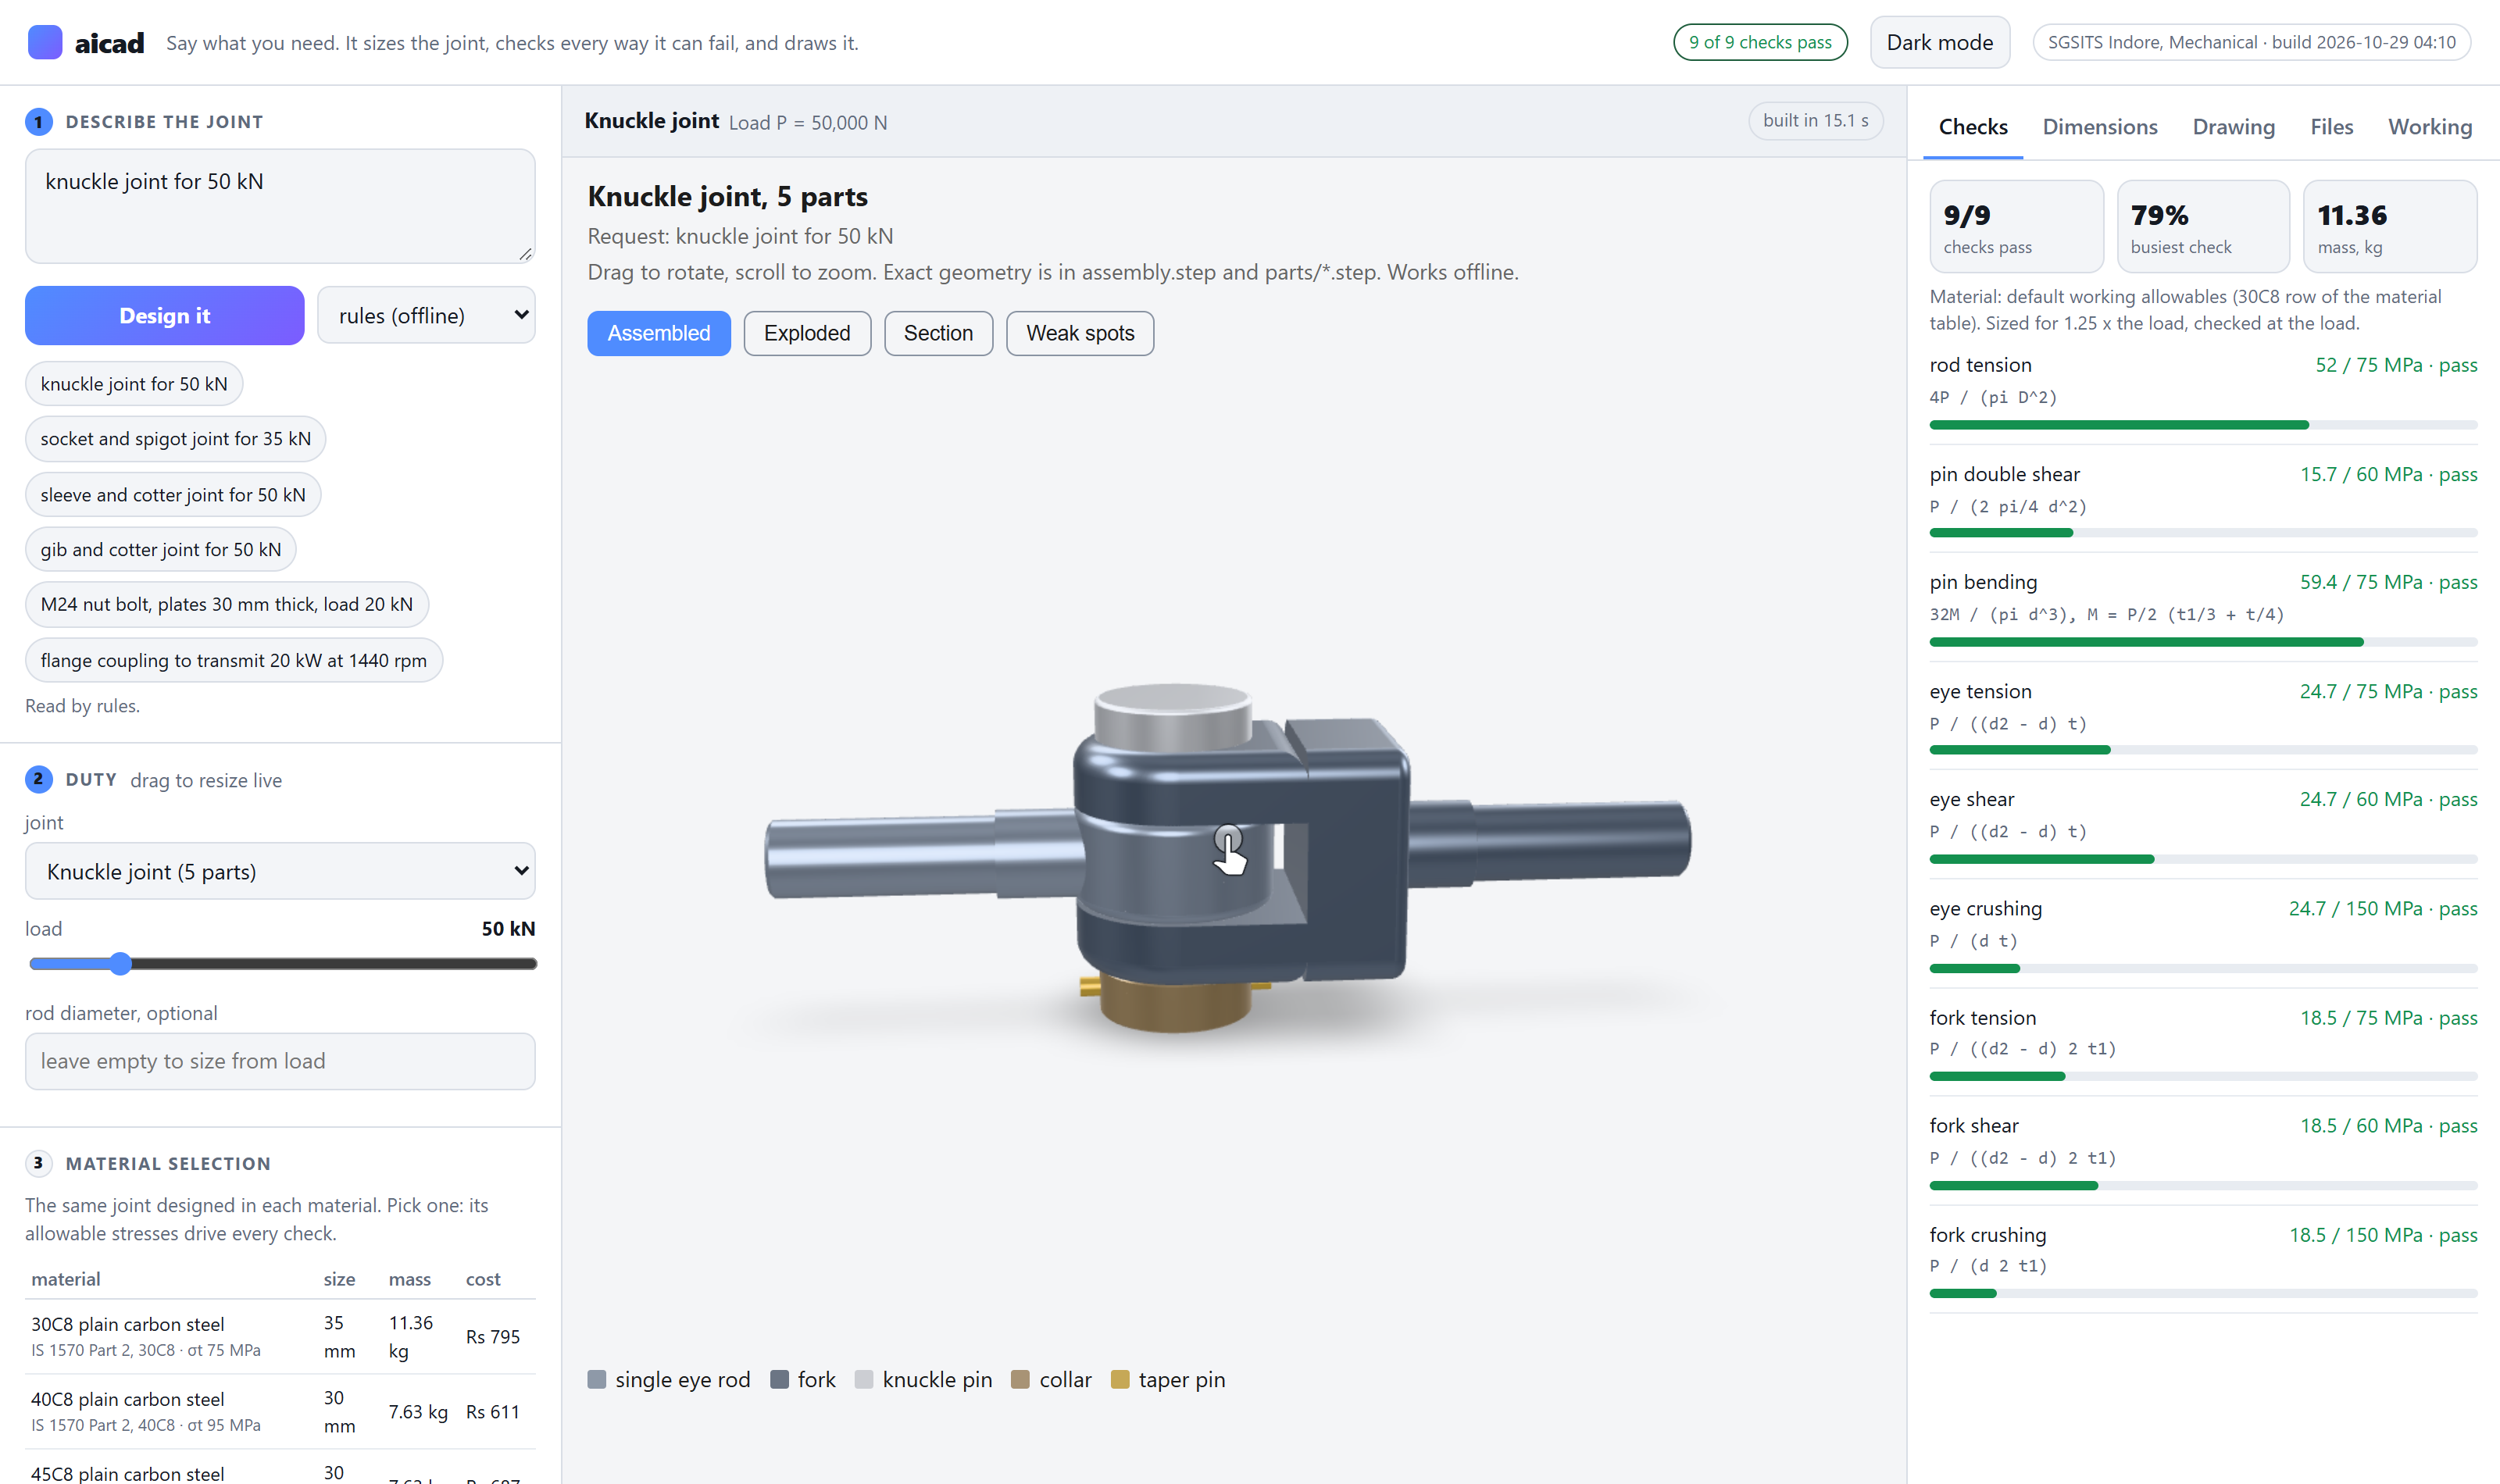
\includegraphics[width=\textwidth,keepaspectratio]{fig/landing.png}\caption{The web application after a design: requirement and sliders, material selection, 3D model, and failure checks}\label{fig:landing}\end{figure}

\section{Build Time}
The time taken by each stage of a build was measured. Sizing and the nine failure checks take under 1 ms, and the solid models take about 0.9 s. The drawing sheet produced by FreeCAD accounts for about 33 s of the 35 s build. Three changes follow from this measurement. The model and the failure checks are now returned first, in about 2 to 5 s, while the drawing sheet is produced in the background, so that the user can read the result while the sheet is being drawn. Results are cached per input, so that a repeated request does not repeat the work. The five textbook cases are built in advance.

\section{Verification of the Implementation}
The implementation is covered by 301 automated tests, which are executed on every change. They cover the sizing arithmetic, the generated geometry, the interpretation of requirements, the drawing sheet, the web interface and the finite element facility. Among them are tests which assert the results printed in the textbook problems, and tests which assert that the source discrepancies recorded in Chapter~7 are genuine, so that the system cannot subsequently be altered to reproduce the printed answers without a test failing.

One class of test detected an error that no dimensional check could have detected. The geometry tests compare the solids of every pair of components and require that no two occupy the same space. That test found a hooked gib modelled 1.25 mm inside the strap, an error invisible in the dimension list because every individual dimension was correct.
}{\chapter{Implementation}}
\IfFileExists{ch7.tex}{\chapter{Results and Discussion}

\section{Design Results}
All six joints size correctly, satisfy every applicable failure check, generate every component as a solid model and produce a drawing sheet. Each design completes in approximately ten seconds. Table~\ref{tab:joints} summarises the results.

\begin{table}[htbp]
\centering\footnotesize
\caption{Design results for the six joints at the duties adopted}\label{tab:joints}
\begin{tabularx}{\textwidth}{>{\raggedright\arraybackslash}X>{\raggedright\arraybackslash}Xrr>{\raggedleft\arraybackslash}p{2.4cm}>{\raggedright\arraybackslash}p{2cm}}
\toprule
Joint & Duty adopted & Parts & Checks & Busiest check, \% of allowable & Outcome \\
\midrule
Knuckle joint & Load P = 50,000 N & 5 & 9 & 79 & all satisfied \\
Socket and spigot cotter joint & Load P = 35,000 N & 3 & 10 & 76 & all satisfied \\
Sleeve and cotter joint & Load P = 50,000 N & 5 & 8 & 77 & all satisfied \\
Gib and cotter joint & Load P = 50,000 N & 4 & 8 & 79 & all satisfied \\
Hex bolt, nut and washer & Load P = 20,000 N & 3 & 2 & 71 & all satisfied \\
Protected type rigid flange coupling & Torque T = 500,000 N mm (500 N m) & 12 & 7 & 79 & all satisfied \\
\bottomrule
\end{tabularx}
\end{table}


The busiest check across the six joints lies between 71 and 79 percent of the allowable stress. That range is the intended consequence of the design factor described in Section~5.4 and confirms that margin is retained in every case.

\section{Worked Example}
The requirement \emph{knuckle joint for 50 kN} is interpreted as the knuckle joint carrying an axial load of 50,000 N with the default allowable stresses. Applying the design factor, the joint is sized for 62,500 N. Table~\ref{tab:raw} gives the governing calculations.

\begin{table}[htbp]
\centering\footnotesize
\caption{Governing calculations for a knuckle joint carrying 50 kN, before rounding}\label{tab:raw}
\begin{tabularx}{\textwidth}{Xrl}
\toprule
Expression & Computed, mm & Effect \\
\midrule
Rod in direct tension & 32.57 & rod diameter adopted as 35 mm \\
Pin in double shear & 25.75 & not governing \\
Pin in bending & 44.85 & governs; pin diameter adopted as 45 mm \\
\bottomrule
\end{tabularx}
\end{table}


The rod requirement of 32.57 mm is rounded up to the adopted 35 mm. The pin requirement arising from bending (44.85 mm, adopted as 45 mm) is about 1.74 times that arising from shear (25.75 mm). A pin sized from shear alone would satisfy its own check and bend in service, which is why the larger of the two requirements is adopted, as the source material does. Table~\ref{tab:dims} gives the complete set of dimensions with the rule and the source behind each.

\begin{table}[htbp]
\centering\scriptsize
\caption{Dimensions computed for the knuckle joint, with the rule behind each}\label{tab:dims}
\begin{tabularx}{\textwidth}{>{\raggedright\arraybackslash}p{1.3cm}>{\raggedright\arraybackslash}p{3.6cm}r>{\raggedright\arraybackslash}X}
\toprule
Symbol & Meaning & Value, mm & Rule and source \\
\midrule
\texttt{D} & rod diameter & 35 & rod in tension: D = sqrt(4P / (pi sigma\_t)), rounded up to a preferred size \\
\texttt{d} & pin diameter & 45 & governed by pin bending \\
\texttt{d2} & eye outer diameter & 90 & d2 = 2.0 x d, the pin diameter (outer diameter of eye and fork, d0 = 2d), rounded up to a standard size [Bhandari, Design of Machine Elements, sec 4.12, eq 4.26j] \\
\texttt{d3} & pin head and collar diameter & 70 & d3 = 1.5 x d, the pin diameter (pin head and collar diameter, 1.5d), rounded up to a standard size [Bhandari, Design of Machine Elements, sec 4.12, eq 4.26o] \\
\texttt{D1} & enlarged end, 1.1D & 40 & D1 = 1.1 x D, the rod diameter (enlarged rod diameter near the eye and fork, D1 = 1.1D), rounded up to a standard size [Bhandari, Design of Machine Elements, sec 4.12, eq 4.26b] \\
\texttt{t} & eye thickness & 45 & t = 1.25 x D, the rod diameter (thickness of eye of rod B, b = 1.25D), rounded up to a standard size [Bhandari, Design of Machine Elements, sec 4.12, eq 4.26n] \\
\texttt{t1} & fork plate thickness & 30 & t1 = 0.75 x D, the rod diameter (thickness of each fork eye, a = 0.75D), rounded up to a standard size [Bhandari, Design of Machine Elements, sec 4.12, eq 4.26m] \\
\texttt{t2} & pin head thickness & 18 & t2 = 0.5 x D, the rod diameter (thickness of pin head), rounded up to a whole mm [NPTEL IIT KGP M4L2 fig 4.2.3.1] \\
\texttt{collar\_t} & collar thickness & 23 &  \\
\texttt{taper\_d} & taper pin diameter (big end) & 9 &  \\
\bottomrule
\end{tabularx}
\end{table}


With all dimensions determined, the nine failure modes are evaluated at the actual load of 50,000 N. The results are given in Table~\ref{tab:checks}. Every check is satisfied, and the busiest, bending of the pin, reaches 79 percent of its allowable stress.

\begin{table}[htbp]
\centering\footnotesize
\caption{Failure checks for the knuckle joint, evaluated at the actual load of 50 kN}\label{tab:checks}
\begin{tabularx}{\textwidth}{>{\raggedright\arraybackslash}p{2.4cm}>{\raggedright\arraybackslash}Xrrr>{\raggedright\arraybackslash}p{1.2cm}}
\toprule
Failure mode & Expression & Stress, MPa & Allowable, MPa & Utilisation, \% & Result \\
\midrule
rod tension & \texttt{4P / (pi D\^{}2)} & 51.969 & 75 & 69 & safe \\
pin double shear & \texttt{P / (2 pi/4 d\^{}2)} & 15.719 & 60 & 26 & safe \\
pin bending & \texttt{32M / (pi d\^{}3), M = P/2 (t1/3 + t/4)} & 59.3829 & 75 & 79 & safe \\
eye tension & \texttt{P / ((d2 - d) t)} & 24.6914 & 75 & 33 & safe \\
eye shear & \texttt{P / ((d2 - d) t)} & 24.6914 & 60 & 41 & safe \\
eye crushing & \texttt{P / (d t)} & 24.6914 & 150 & 16 & safe \\
fork tension & \texttt{P / ((d2 - d) 2 t1)} & 18.5185 & 75 & 25 & safe \\
fork shear & \texttt{P / ((d2 - d) 2 t1)} & 18.5185 & 60 & 31 & safe \\
fork crushing & \texttt{P / (d 2 t1)} & 18.5185 & 150 & 12 & safe \\
\bottomrule
\end{tabularx}
\end{table}


\begin{landscape}
\begin{figure}
\centering
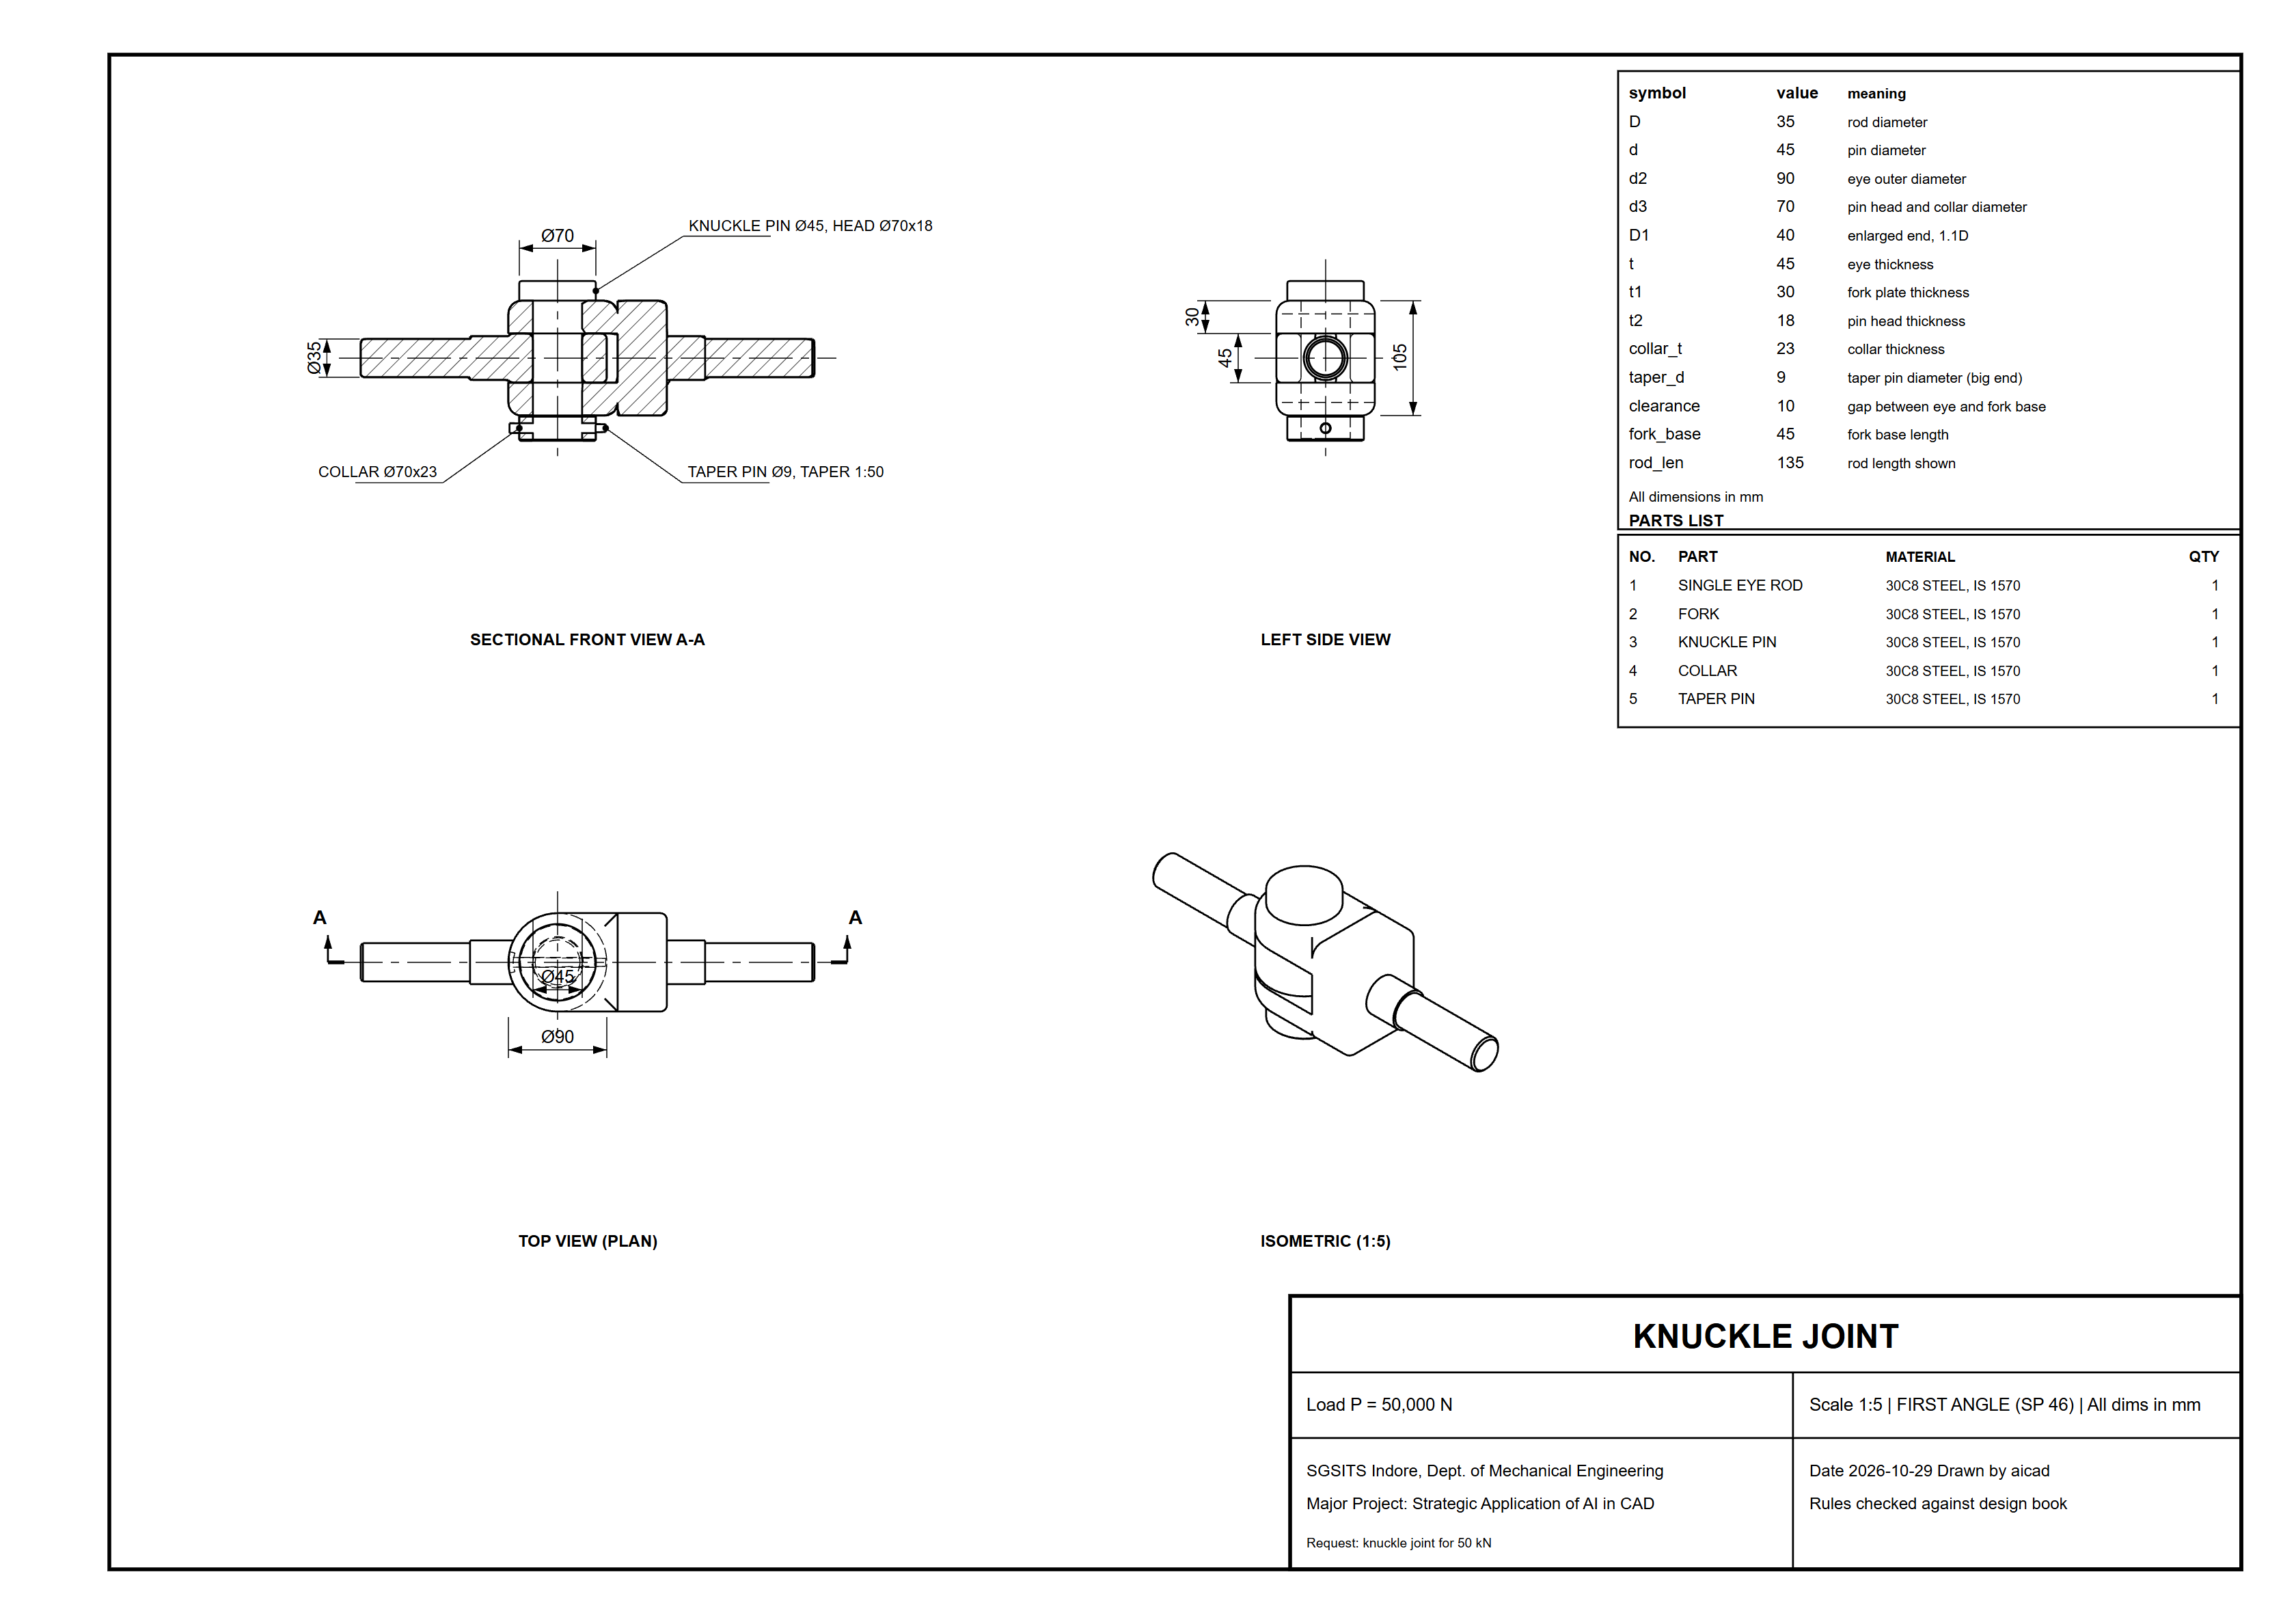
\includegraphics[width=\linewidth,height=0.94\textheight,keepaspectratio]{fig/drawing.png}
\caption{First angle A3 drawing sheet for the knuckle joint of Section 7.2: sectional front view A-A, side view, plan, isometric, parts list}
\label{fig:drawing}
\end{figure}
\end{landscape}

\begin{figure}
\centering
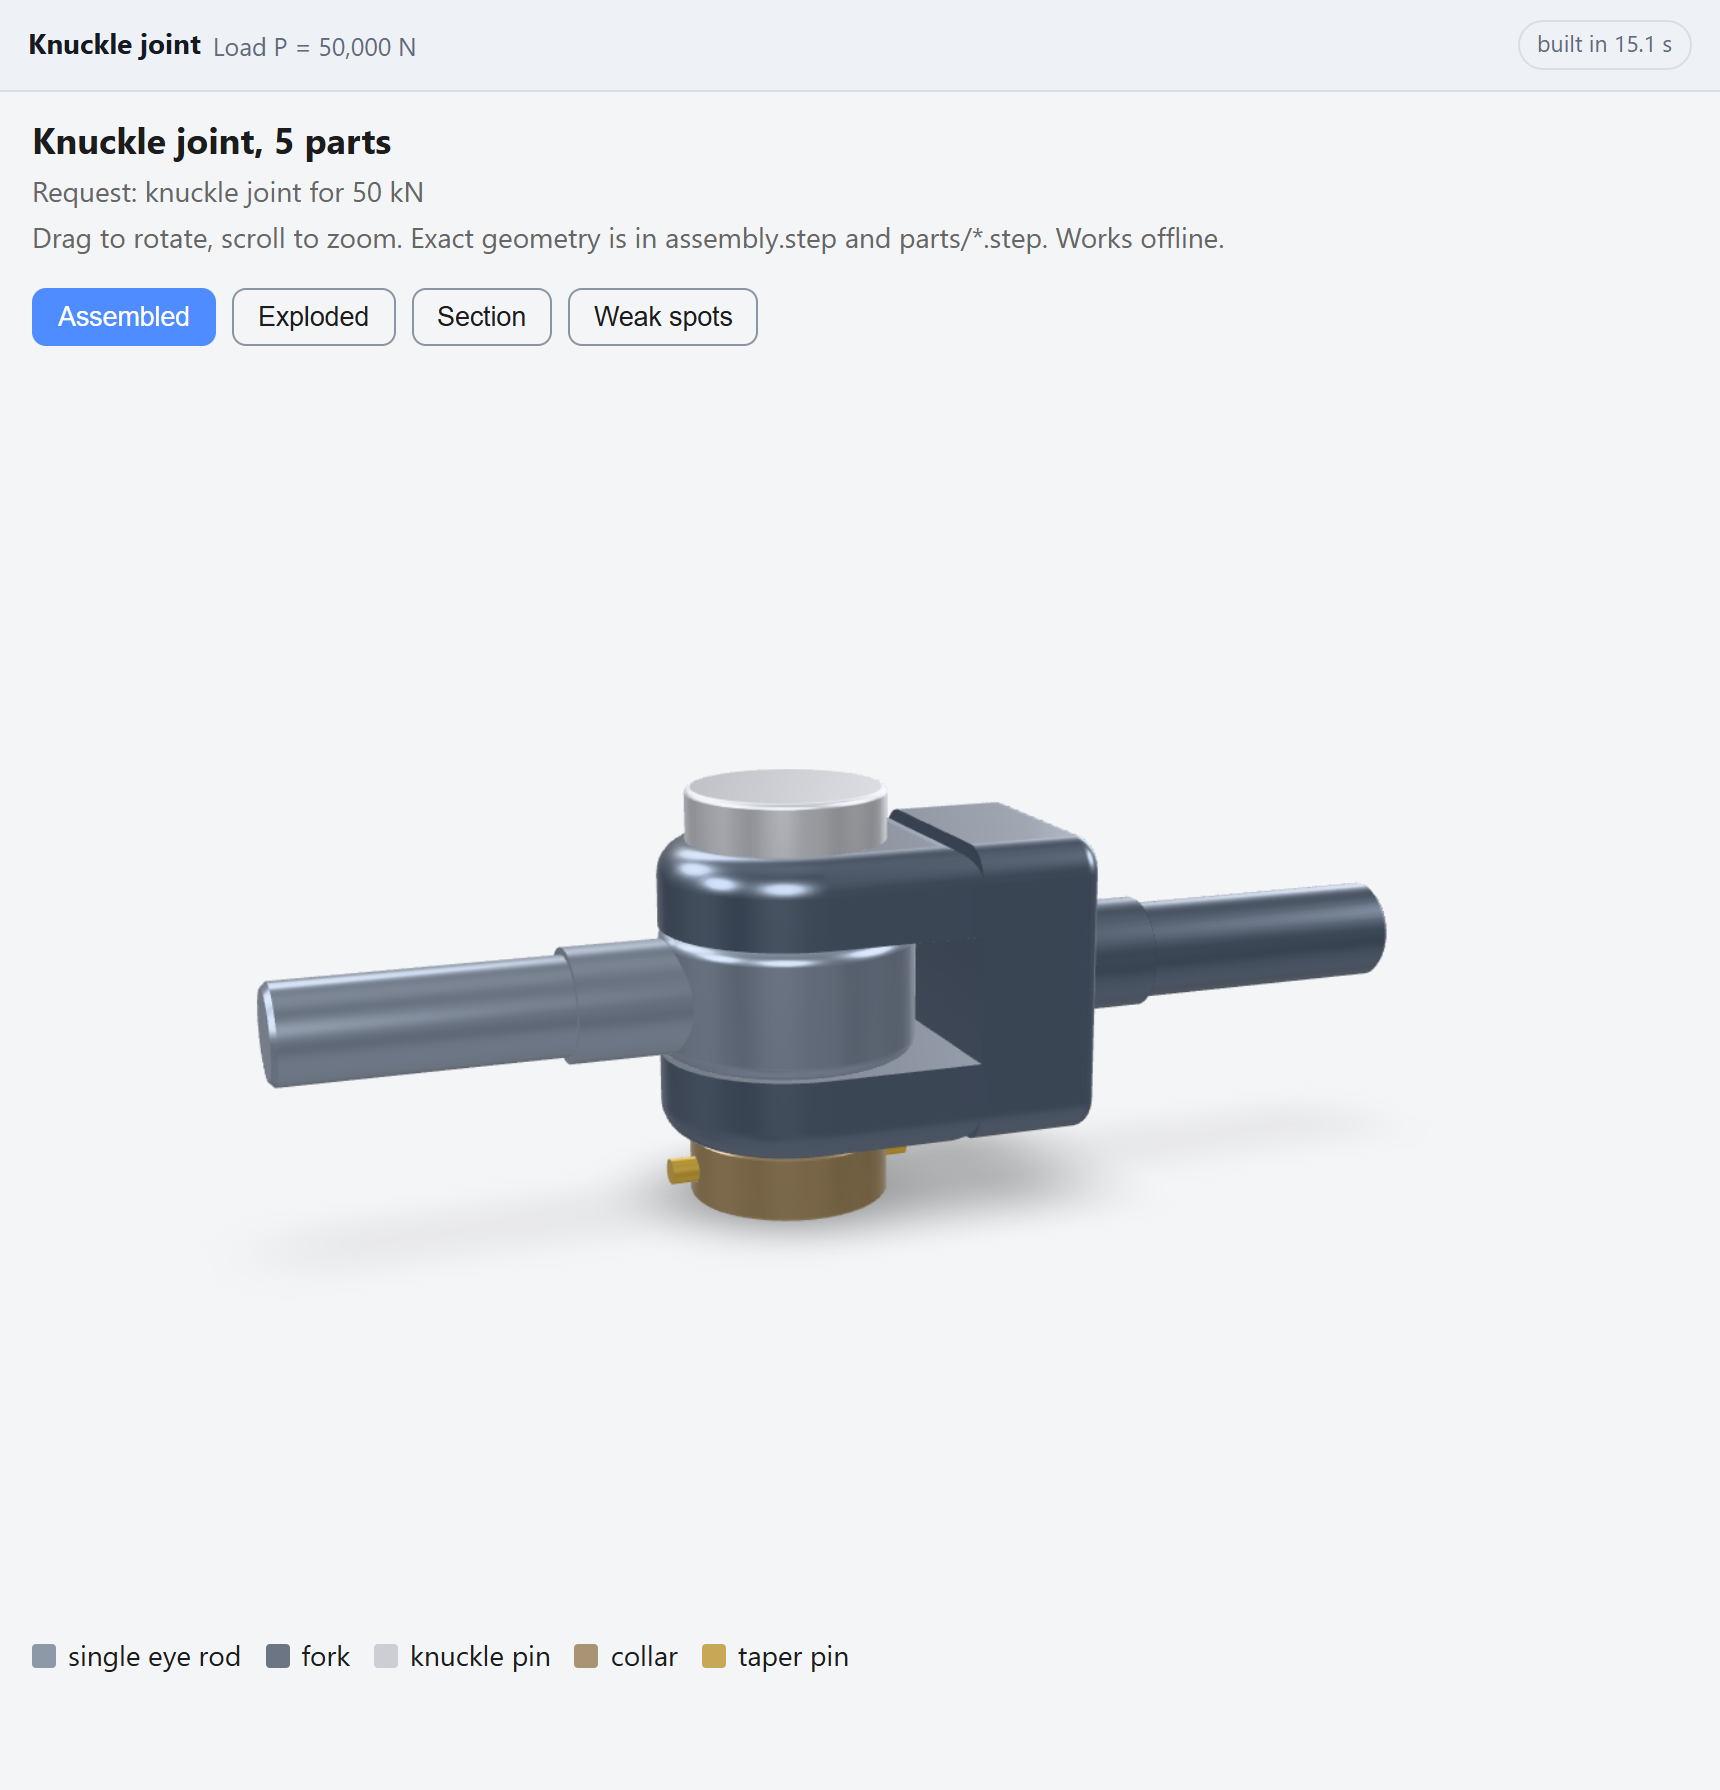
\includegraphics[width=0.62\textwidth]{fig/model.png}
\caption{Assembled model of the same joint, also available exploded and coloured by utilisation}
\label{fig:model}
\end{figure}

\section{Verification Against Published Literature}
Every proportion and every failure check was compared against the sources reviewed in Chapter~2. The outcome for each joint is given in Table~\ref{tab:verify}.

\begin{table}[htbp]
\centering
\caption{Verification of each joint against published design literature}
\label{tab:verify}
\small
\begin{tabularx}{\textwidth}{@{}lXX@{}}
\toprule
Joint & Source consulted & Outcome \\
\midrule
Knuckle joint & Bhandari Ex 4.5 and Problem 4.1; NPTEL Module 4 Lesson 2 & Sizes and stresses of Ex 4.5 reproduced exactly; all checks verified \\
Socket and spigot cotter & Bhandari Ex 4.2; NPTEL Module 4 Lesson 2; Leutwiler Art.\ 98 & Nine of ten sizes reproduced; checks verified against two sources \\
Gib and cotter & Unwin, p.\ 179 & Breadth division, thickness and taper verified \\
Protected flange coupling & NPTEL Module 4 Lesson 1; Leutwiler Art.\ 275 & All checks verified twice; proportions not verifiable \\
Sleeve and cotter & Four sources searched, none covers it & Checks verified by correspondence; proportions unverified \\
Hex bolted joint & NPTEL Module 4 Lesson 4 & Tightening relation verified; size table unverified \\
\bottomrule
\end{tabularx}
\end{table}

Two entries require explanation. For the flange coupling, the failure checks are verified against two independent sources, but the empirical proportions are marked unverified. This is not an omission. As recorded in Section~2.2, Leutwiler states that no standard set of proportions was ever agreed and that published tables reflect the practice of individual manufacturers. The proportions are therefore a convention, and the system reports them as such on every run. For the sleeve and cotter joint, none of four sources treats the joint by name; its checks are verified by direct correspondence with the socket and spigot cotter joint, but its proportions remain unsupported and are reported as such.

The strongest test is the reproduction of complete worked examples. Given the inputs of Bhandari's Example 4.5, the software adopts all seven sizes the book adopts and computes the same six eye and fork stresses, 31.25 and 25 N/mm\textsuperscript{2}. Table~\ref{tab:bhandari} sets the two side by side.

\begin{table}[htbp]
\centering\footnotesize
\caption{Bhandari Example 4.5 (50 kN, 30C8, factor of safety 5) against the software run with the same inputs}\label{tab:bhandari}
\begin{tabularx}{\textwidth}{llrrl}
\toprule
Quantity & Meaning & Book & Software & Agrees \\
\midrule
\texttt{D} & rod diameter & 30 & 30 & yes \\
\texttt{D1} & enlarged end, 1.1D & 35 & 35 & yes \\
\texttt{t} & eye thickness & 40 & 40 & yes \\
\texttt{t1} & fork plate thickness & 25 & 25 & yes \\
\texttt{d} & pin diameter & 40 & 40 & yes \\
\texttt{d2} & eye outer diameter & 80 & 80 & yes \\
\texttt{d3} & pin head and collar diameter & 60 & 60 & yes \\
eye tension & stress, MPa & 31.25 & 31.25 & yes \\
fork tension & stress, MPa & 25 & 25 & yes \\
\bottomrule
\end{tabularx}
\end{table}


Problem 4.1 is reproduced to the printed 14.47 mm for the rod and 13.47 mm for the pin. For the cotter joint of Example 4.2, nine of the ten adopted sizes agree, including the spigot and socket diameters solved from their tension equations (37.91 and 52.04 mm before rounding). The one difference, the width of the cotter, follows from the book designing the cotter alone with a factor of safety of 4 while the software applies the factor of the rods to every part. Each of these cases is an automated test and a one click case in the web application.

The two texts also disagree on one proportion of the knuckle joint. The NPTEL lesson takes the pin head as 1.5 times the rod diameter, which gives 60 mm on its own 55 mm pin, a head only 5 mm larger than the pin. Bhandari takes it as 1.5 times the pin diameter. The software follows Bhandari.

\section{Discrepancies Found in the Sources}
The verification exercise identified three errors in the published sources. They are recorded here because the behaviour of the system deliberately differs from the printed material in consequence.

\subsection{A Worked Example That Fails Its Own Check}
The NPTEL knuckle joint problem raises the pin diameter from 40 mm to 55 mm to satisfy bending, but then evaluates the eye using the original 40 mm pin. Evaluated with the pin actually adopted, its own expression for shear of the eye gives 80 MPa against an allowable of 65 MPa, an exceedance of 23 percent. The present system instead enlarges the outer diameter of the eye and reports that it has done so.

\subsection{An Omitted Failure Mode}
The NPTEL cotter joint procedure verifies crushing of the socket but not crushing between the cotter and the spigot. Evaluated at the final answer of that source, the omitted check gives 167 MPa against an allowable of 110 MPa. Leutwiler, in Article 98, lists this mode among ten, with an expression of identical form. The present system retains the check and sizes the cotter thicker in consequence. That an independent text, published eighteen years earlier, lists a check which the lesson omits establishes this as an omission rather than a matter of preference.

\subsection{A Constant Printed Incorrectly}
The initial tightening load for a bolted joint is printed as $284d$ kN. The worked example on the same page obtains 56.8 kN for an M20 bolt, which is consistent only with a constant of $2840d$ N. The printed relation is therefore in error by a factor of one hundred, and the source refutes itself. The system uses $2840d$ N and reports the tightening load on every bolted design.

\section{Finite Element Comparison}
The finite element facility was first validated against a case with a known answer. Table~\ref{tab:fe} gives the comparison, measured on the September geometry.

\begin{table}[htbp]
\centering
\caption{Comparison of the finite element result with the calculated stress}
\label{tab:fe}
\small
\begin{tabularx}{\textwidth}{@{}>{\raggedright\arraybackslash}Xrrr@{}}
\toprule
Case & Formula, MPa & FEA, MPa & Diff., \% \\
\midrule
Bar of 20 mm diameter, 10 kN in tension & 31.83 & 32.22 & $+1.2$ \\
Knuckle joint eye rod, 50 kN & 52.0 & 57.9 & $+11.3$ \\
\bottomrule
\end{tabularx}
\end{table}

The bar validates the method. The eye rod reads higher because the calculation treats the rod as a plain bar in tension and takes no account of the stress raised at the pin bore, whereas the finite element model does. Both values remain below the allowable stress of 75 MPa.

The convergence rule described in Section~5.7 proved necessary in practice. For one component the computed peak varied from 157 to 191 MPa across a sixteen fold increase in the number of nodes without settling, which indicates a singularity at the constrained face rather than a physical stress. The system reports such a result as not converged and directs the user to the calculated value.

\section{Discussion}
The division of responsibility of Section~5.2 gave a natural language interface without making any part of the design unverifiable, and printing the arithmetic of every check is what exposed the three discrepancies of Section~7.4: each surfaced because a computed number disagreed with a printed one.

\section{Objectives Revisited}
\begin{enumerate}
\item \textbf{Interpreting a plain English requirement.} Met. The language model extracts the joint type and load, as shown in Section~5.2, and any value it returns that cannot be traced back to the original sentence is discarded, which guards against a fabricated input.
\item \textbf{Sizing and verifying against every failure mode, with iteration.} Met. All six joints satisfy every applicable check at the stated load, as given in Table~\ref{tab:joints}, and the iterative enlargement of Section~5.5 is what makes the gib and cotter strap, and the knuckle eye of the NPTEL problem, pass where the source proportions alone would not.
\item \textbf{Exact solid models in a neutral format that opens in commercial CAD software.} Substantially met. Every exported assembly was inspected directly and confirmed to carry the AUTOMOTIVE\_DESIGN (AP214) schema with each component as a separate named solid rather than a single fused body, which is the structure Siemens NX requires to recognise an assembly on import. Opening the file inside NX itself, available only in the departmental laboratory, is the one point not yet confirmed by direct observation and is recorded as such.
\item \textbf{A first angle drawing sheet conforming to Indian practice.} Met for projection and sheet layout, as shown in Figure~\ref{fig:drawing}. Dimensioning to SP 46 tolerance and surface finish conventions is not implemented and is listed in Section~8.2.
\item \textbf{Verification against published literature, with disagreements recorded.} Met for four of six joints and partially met for the remaining two, as tabulated in Table~\ref{tab:verify}. The three discrepancies of Section~7.4 are the direct product of this objective rather than a side finding.
\item \textbf{Browser use without installation.} Met. The system is deployed and reachable without a local install, though the hosted copy runs the rule based interpreter rather than the language model, a distinction recorded in Section~5.2.
\end{enumerate}

}{\chapter{Results and Discussion}}
\IfFileExists{ch8.tex}{\chapter{Conclusions and Scope of Future Work}

\section{Conclusions}

A system has been developed which accepts a machine joint requirement written in ordinary English and returns a complete design. Every dimension is computed from published design formulas, every applicable failure mode is verified against the allowable stress, every component is generated as an exact solid model, and a first angle sectional drawing is produced with dimensions, a parts list and a title block. Six joints are implemented, applying 44 distinct failure checks in total, and the implementation is covered by 301 automated tests. A material selection step offers six materials and accepts the user's own.

The objective of keeping the design traceable has been met. Every dimension can be attributed either to a formula with a cited source or to an explicitly named failure check, and the working of each run is printed in full so that the result can be verified rather than accepted.

The system was validated against worked examples from the reference text. The knuckle joint reproduces Bhandari Example 4.5 exactly, and the cotter joint reproduces nine of the ten sizes of Example 4.2. The exercise also revealed three errors in the sources themselves, one of which is a worked example whose own answer exceeds its allowable stress by 23 percent. These were found because the system evaluates every check on every design and reports the arithmetic. The division of responsibility, in which the language model reads the requirement and deterministic code does the engineering, is the element most generally applicable beyond these joints.

\section{Scope for Future Work}

\begin{enumerate}
  \item \textbf{Additional joints.} Riveted and welded joints follow the same pattern and could be added without change to the architecture.
  \item \textbf{Fatigue loading.} All sizing at present is static. An endurance limit and a stress concentration factor would extend the system to cyclically loaded joints.
  \item \textbf{Tolerances, fits and GD\&T.} The sheet carries nominal dimensions only. Fits, tolerances and geometric dimensioning and tolerancing would make it directly usable for manufacture.
  \item \textbf{Verification of remaining proportions.} Three joints have proportions without a supporting source: the sleeve and cotter joint, the flange coupling and the hex bolt size table. A design data handbook would settle all three.
  \item \textbf{NX journal.} A journal script for Siemens NX would build the assembly within that software instead of importing STEP.
  \item \textbf{Cotter factor of safety and costing.} A separate factor of safety for the cotter, as Bhandari uses, and a costed bill of materials.
\end{enumerate}
}{\chapter{Conclusions and Scope of Future Work}}

% ----------------------------------------------------------------- appendices
\clearpage
\phantomsection\addcontentsline{toc}{chapter}{Appendix A \quad Screenshots of the Working System}
\markboth{Appendix A}{}\expandafter\gdef\csname tp@\thepage\endcsname{}
\begingroup
\singlespacing
\begin{center}{\fontsize{14}{17}\selectfont\bfseries APPENDIX A\\ SCREENSHOTS OF THE WORKING SYSTEM}\end{center}
\vspace{-2mm}
\noindent\begin{minipage}{0.14\textwidth}
\includegraphics[width=\linewidth]{fig/demo-qr.png}\end{minipage}\hfill
\begin{minipage}{0.83\textwidth}\small The system is deployed and can be used without installation at
\mbox{\textbf{aicad-vercel.vercel.app}}. Scan the code or enter the address in a browser; the screenshots
below were captured from it.\end{minipage}

\renewcommand{\thefigure}{A.\arabic{figure}}
\setcounter{figure}{0}
\begin{figure}[htbp]
\centering
\begin{subfigure}[t]{0.49\textwidth}\centering
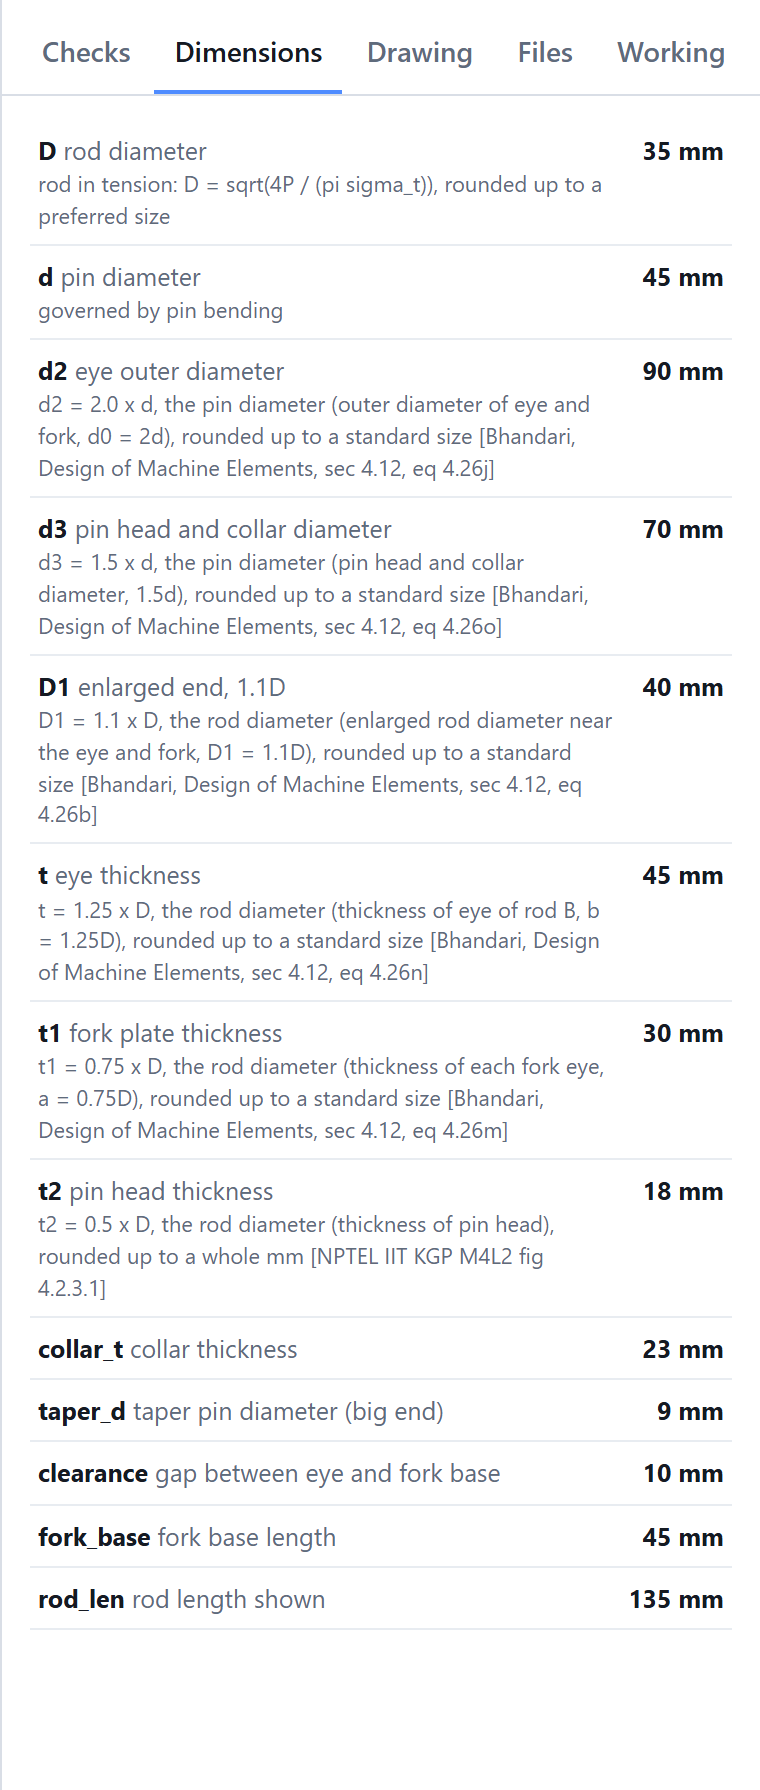
\includegraphics[height=0.32\textheight,width=\linewidth,keepaspectratio]{fig/dimensions.png}
\caption{Computed dimensions with rule and source}\end{subfigure}\hfill
\begin{subfigure}[t]{0.49\textwidth}\centering
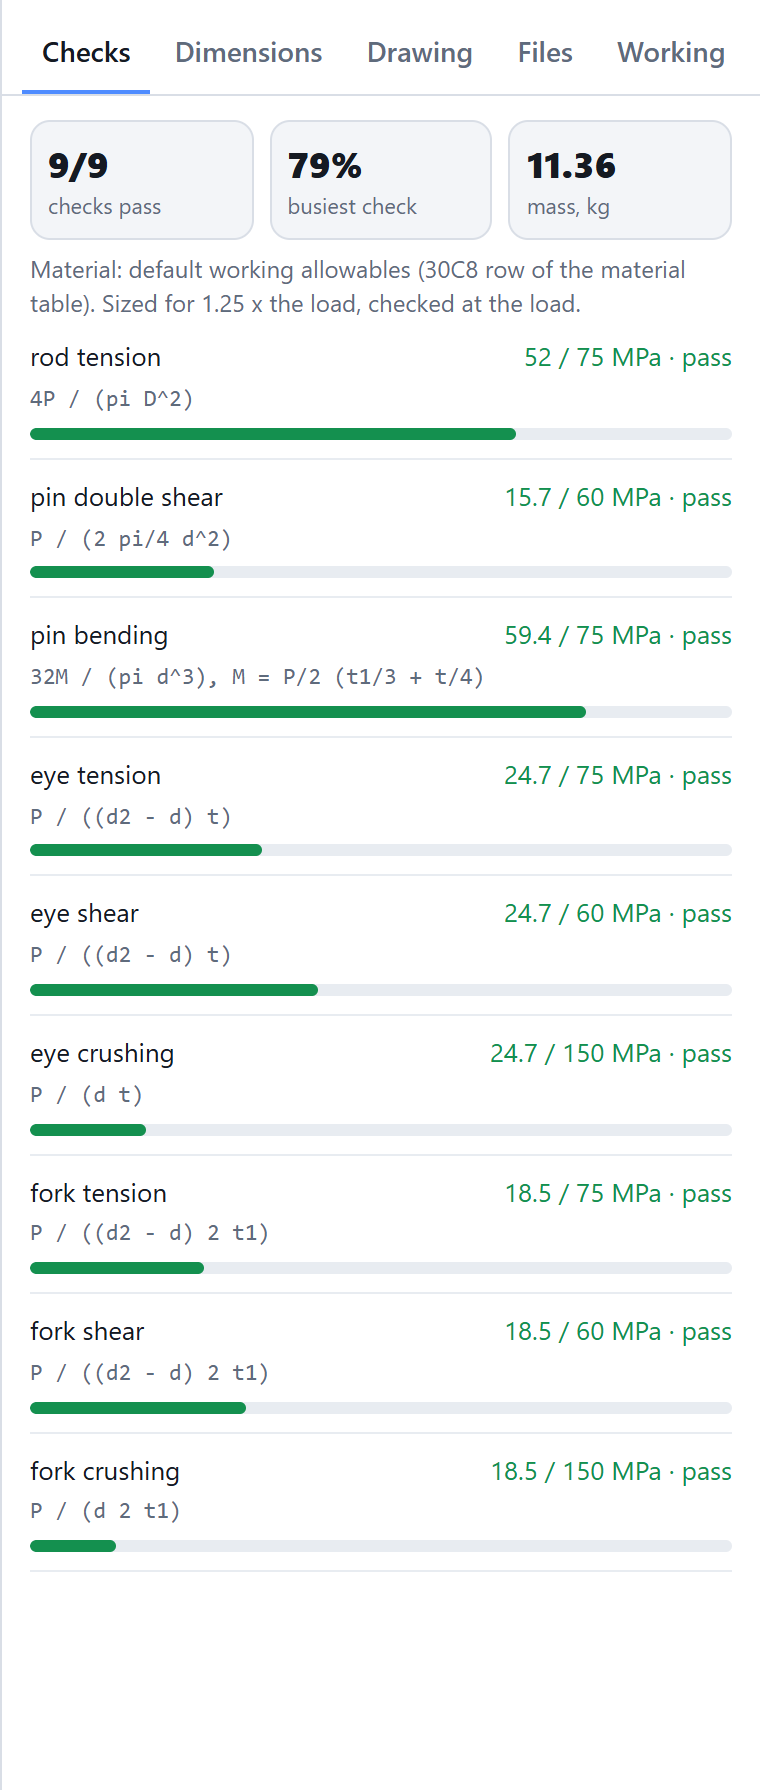
\includegraphics[height=0.32\textheight,width=\linewidth,keepaspectratio]{fig/checks.png}
\caption{Failure checks with substituted arithmetic}\end{subfigure}\\[2mm]
\begin{subfigure}[t]{0.49\textwidth}\centering
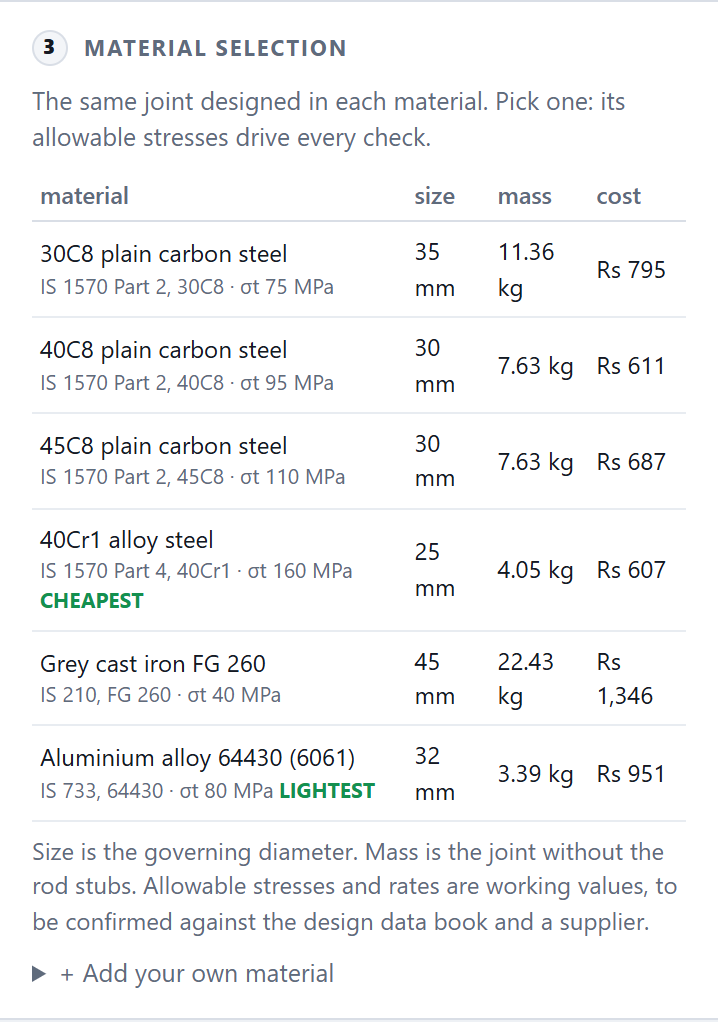
\includegraphics[height=0.32\textheight,width=\linewidth,keepaspectratio]{fig/materials.png}
\caption{Material selection}\end{subfigure}\hfill
\begin{subfigure}[t]{0.49\textwidth}\centering
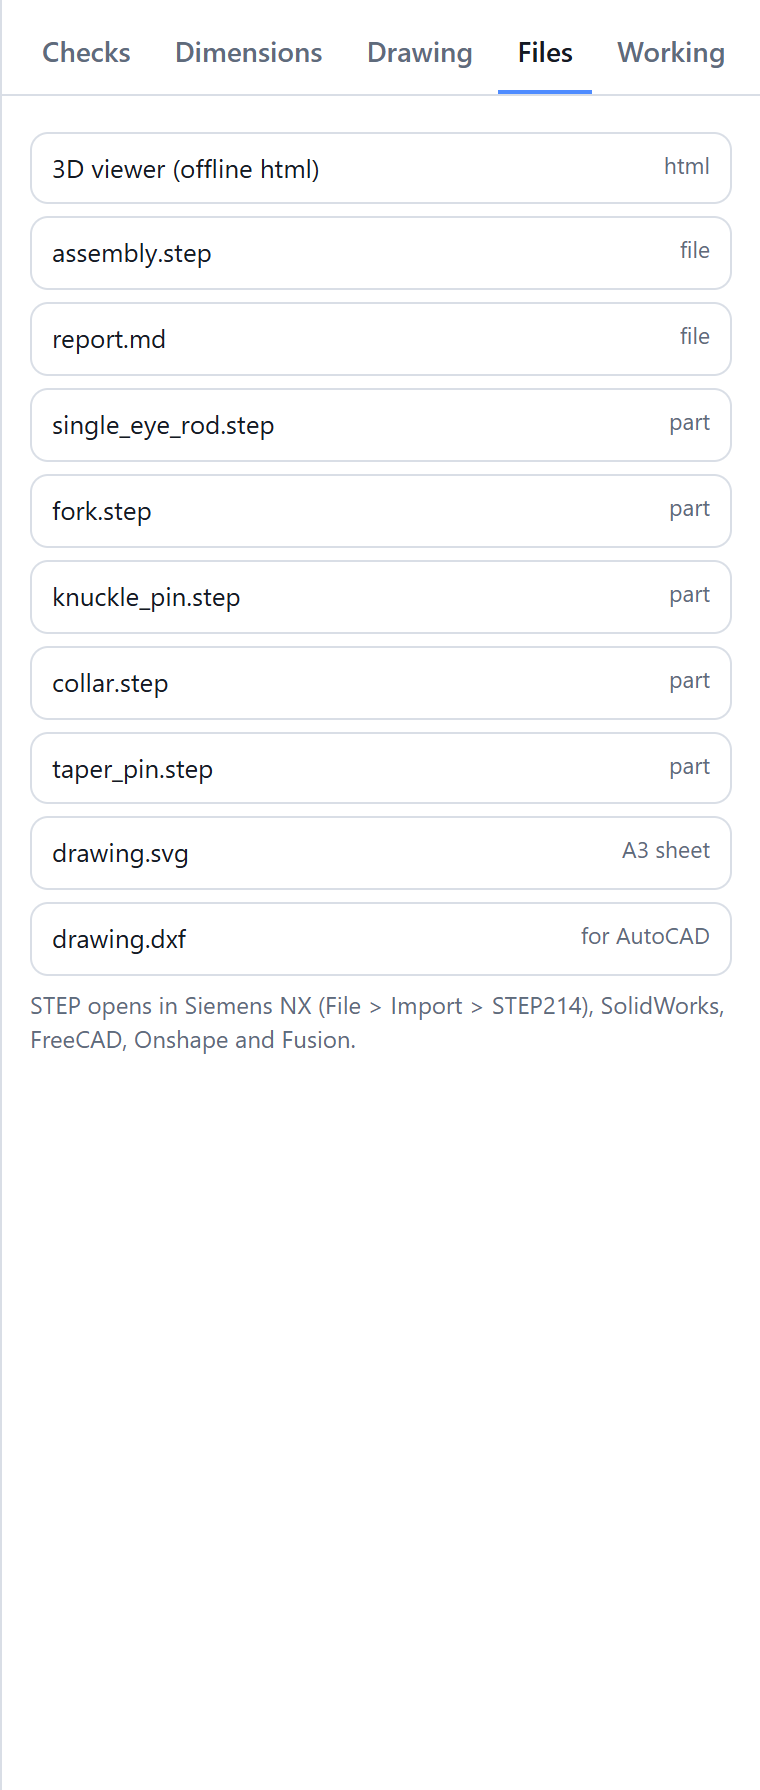
\includegraphics[height=0.32\textheight,width=\linewidth,keepaspectratio]{fig/files.png}
\caption{Files produced by a run}\end{subfigure}
\caption{Screenshots of the deployed system}\label{fig:appA}
\end{figure}
\endgroup

\clearpage
\phantomsection\addcontentsline{toc}{chapter}{Appendix B \quad Selected Source Code}
\markboth{Appendix B}{}\expandafter\gdef\csname tp@\thepage\endcsname{}
\begin{center}{\fontsize{14}{17}\selectfont\bfseries APPENDIX B\\ SELECTED SOURCE CODE}\end{center}
\singlespacing\small\noindent The listings are read from \texttt{aicad/joints/knuckle.py} when the
report is generated. The complete source is at github.com/Atishyy27/aicad.
\begingroup
\renewcommand{\lstlistingname}{Listing B.}\renewcommand{\thelstlisting}{\arabic{lstlisting}}
\lstinputlisting[caption={Sizing the knuckle joint from the load (\texttt{design}, trimmed to the sizing lines)},captionpos=t]{listings/knuckle_sizing.txt}
\lstinputlisting[caption={The nine failure checks of the knuckle joint (\texttt{\_checks})},captionpos=t]{listings/knuckle_checks.txt}
\endgroup


% ----------------------------------------------------------------- references
\clearpage\phantomsection\addcontentsline{toc}{chapter}{References}
\markboth{References}{}
\fmhead{REFERENCES}
\singlespacing\footnotesize
\begin{list}{}{\setlength{\leftmargin}{9mm}\setlength{\labelwidth}{9mm}\setlength{\itemsep}{2pt}\setlength{\parsep}{0pt}}
\item[{[1]}] Indian Institute of Technology Kharagpur. Design of Machine Elements I, Module 4: Fasteners and Joints. National Programme on Technology Enhanced Learning; Lessons 1 to 4.
\item[{[2]}] Bhandari VB. Design of Machine Elements. New Delhi: McGraw Hill Education; Chapter 4, sections 4.9 to 4.12, Examples 4.2 to 4.5 and Problem 4.1.
\item[{[3]}] Unwin WC. The Elements of Machine Design, Part I. London: Longmans, Green and Co.; 1899. Article 103 and Figures 130 and 131, page 179.
\item[{[4]}] Leutwiler OA. Elements of Machine Design. New York: McGraw Hill Book Company; 1917. Article 98, pages 122 to 124; Article 275, pages 383 to 386.
\item[{[5]}] IS 2048: Parallel Keys and Keyways. New Delhi: Bureau of Indian Standards.
\item[{[6]}] IS 1363 and IS 1364: Hexagon Head Bolts, Screws and Nuts. New Delhi: Bureau of Indian Standards.
\item[{[7]}] IS 2693: Cast Iron Flange Couplings. New Delhi: Bureau of Indian Standards.
\item[{[8]}] SP 46: Engineering Drawing Practice for Schools and Colleges. New Delhi: Bureau of Indian Standards.
\item[{[9]}] Open Cascade SAS. Open CASCADE Technology geometric modelling kernel. \url{https://dev.opencascade.org/} (Accessed on September 20, 2026).
\item[{[10]}] CadQuery Developers. CadQuery 2.8, parametric modelling library for Python. \url{https://cadquery.readthedocs.io/} (Accessed on September 20, 2026).
\item[{[11]}] FreeCAD Developers. FreeCAD, an open source parametric CAD application; TechDraw workbench. \url{https://www.freecad.org/} (Accessed on September 21, 2026).
\item[{[12]}] Dhondt G. CalculiX: A Three Dimensional Structural Finite Element Program. \url{http://www.calculix.de/} (Accessed on September 21, 2026).
\item[{[13]}] Geuzaine C, Remacle JF. Gmsh: a three dimensional finite element mesh generator with built in pre and post processing facilities. International Journal for Numerical Methods in Engineering. 2009; 79(11):1309--1331.
\item[{[14]}] BuildCAD AI. Text and photo to 3D model generator. \url{https://buildcad.ai/} (Accessed on October 29, 2026).
\item[{[15]}] Zoo. Text-to-CAD. \url{https://zoo.dev/} (Accessed on October 29, 2026).
\item[{[16]}] CADAM (Adam). Open source text to parametric OpenSCAD. \url{https://adam.new/} (Accessed on October 29, 2026).
\item[{[17]}] Leo AI. Engineering copilot. \url{https://getleo.ai/} (Accessed on October 29, 2026).
\item[{[18]}] MITCalc. Mechanical, industrial and technical calculations. \url{https://mitcalc.com/} (Accessed on October 29, 2026).
\item[{[19]}] KISSsoft. Software for the sizing and analysis of machine elements. \url{https://www.kisssoft.com/} (Accessed on October 29, 2026).
\item[{[20]}] Khan MS, Sinha S, Uddin T, Stricker D, Ali SA, Afzal MZ. Text2CAD: Generating Sequential CAD Models from Beginner-to-Expert Level Text Prompts. Advances in Neural Information Processing Systems 37 (NeurIPS 2024).

\end{list}
\end{document}
